% D04-001. AI-01 P0064--P0092, уточнения по локальным реализациям.
\section{Архитектуры нейросетей для анализа осциллограмм}
\label{sec:ch4_physkan_architectures}

При анализе осциллограмм нейронная сеть должна выделять признаки
процесса из сигналов токов и напряжений. Выбор архитектуры определяет,
какие связи между этими сигналами задаются заранее, а какие должны
быть установлены в ходе обучения. Для задач РЗА представляет интерес
введение в вычисления известных электротехнических соотношений.
Они дают исходную структуру для обработки сигналов, а обучаемая часть
позволяет учитывать особенности зарегистрированных процессов.

В настоящей работе обозначение ФизКАН объединяет разрабатываемые
модификации нейронных сетей с физически мотивированными цепочками,
различными реализациями KAN и их сочетаниями. Развитие этого подхода
рассматривается на примере вещественной модели PhysicsKAN,
комплексной cPhysicsKAN и модели rPhysicsKAN с управлением
амплитудными признаками по фазовым соотношениям.\footnote{Евдаков А.Е.
Архитектурная модернизация интеллектуальных алгоритмов релейной защиты.
Внедрение законов электротехники в граф вычислений.}
Эти варианты отражают различные способы включения физической
информации в обработку осциллограммы.


\iffalse
(Примечание автора: введение не совсем в моей редакции. 
Прост его надо смотреть не только на основе первой статьи. 
И возможно сейчас ты точно не знаешь, как описать – поэтому будет тебе прост отложенная задача, которую надо не забыть выполнить. 
Отсюда можешь удалить этот комментарий, прост перенеси в нужное место. 
Можешь постепенно писать даже, если появляются мысли или сделать себе отложенной задачей, тогда аккуратно напиши это тут) **[AA044: закрыто автором; сохранено в истории]**
(Примечание автора: Тут задача закрыта. Прост добавь примечание чуть другое в введении из серии как делала потом далее, что ещё делается и всё)
\fi
\authorreviewnote{AA044}


\subsection{Входные данные и результат обработки окна}
\label{sec:ch4_input_windows}


\iffalse
(Примечание автора: И подумай всё же куда вынести «Методологию» с расчётами, метриками и прочим. Так как очень важный момент перед всем, а пока что он упущен полностью. И/или ответь мне где именно это будет. Повторять статьи по структурам не обязательно, а вот по тексту того, что затрагивается, хорошо бы. И быть может, разные моменты стоит объединять из разных статей как раз, ибо они важны, но по началу не затрагивались) **[AA045: закрыто автором; сохранено в истории]**
(Примечание автора: Да, всё хорошо, закрывай, только не забудь про РНМ в той главе, сделай пометку.)
\fi
\authorreviewnote{AA045}


Для описания архитектур необходимо сначала определить форму данных,
с которыми работает сеть. Один пример представляет собой ограниченный
фрагмент осциллограммы или подготовленное по нему представление.
Временное окно сохраняет порядок отсчётов и соответствие каналов.
Гармоническое представление содержит выделенные составляющие
сигналов, для которых могут отдельно задаваться амплитуды и фазы.
Выбор такого представления меняет смысл элементов входа
и рассматривается совместно с архитектурой.

При обработке многоканального фрагмента обозначим его матрицу
$X\in\mathbb{R}^{C\times T}$, где $C$ является числом сигналов, например фазных токов
$I_A$, $I_B$, $I_C$ и напряжений $U_A$, $U_B$, $U_C$,
а $T$ числом позиций вдоль обрабатываемой оси. Для временного
представления эта ось соответствует отсчётам. После извлечения
признаков её смысл определяется принятой процедурой подготовки.
\iffalse
(Примечание автора: Проведи сравнение подобных описаний со статьёй, может что-то стоит улучшить, а может и нормально. Прост пока что я вижу излишний математиизм, а точнее не везде его понятность, например строка «где C является числом каналов» - хорошо бы уточнить, что канал, это, например, Ia. А про батчи – возможно и не особо-то нужно здесь, это уже тонкости обучения, ну либо где-то позже вскользь про это уже при самом обучении, ибо тут мы и не размышляем никак об это размерности.) **[AA046: закрыто автором; сохранено в истории]**
(Примечание автора: Да, нормально, закрывай)
\fi
\authorreviewnote{AA046}
Например, один период из шести сигналов, представленный
32 отсчётами каждого сигнала, имеет размер $6\times32$.
\iffalse
(Примечание автора: например 1 период с 32 точками.) **[AA047: закрыто автором; сохранено в истории]**
(Примечание автора: Да, закрывай)
\fi
\authorreviewnote{AA047}
Полносвязный вход
такого окна содержит 192 компоненты. В свёрточной модели
сохраняются две отдельные оси каналов и отсчётов.

На выходе классификатор формирует $K$ числовых оценок,
соответствующих выбранным меткам. Последний линейный слой
в рассматриваемых реализациях не содержит окончательного
порогового решения. Если признаки событий оцениваются независимо,
к выходам может применяться сигмоидальная функция. При выборе
одного класса из взаимно исключающих альтернатив используется
нормировка по совокупности выходов. Поэтому смысл оценки
и способ получения окончательной метки определяются постановкой
задачи, а не только формой последнего слоя.
\iffalse
(Примечание автора: Наверное можно бы добавить какую-то картинку простенькую. И повторюсь, пиши инструкции к картинкам, чтобы потом их отрисовывать, так как я могу это делать через более хороших твоих коллег.) **[AA048: закрыто автором; сохранено в истории]**
(Примечание автора: Да, закрыта)
\fi
\authorreviewnote{AA048}


На рисунке~\ref{fig:ch4_output_decision} показано независимое
получение нескольких меток из оценок модели. Числа и сигналы
на схеме условные. Наличие ОЗЗ и его дугового характера может
определяться совместно, тогда как выход РНМ имеет собственную
целевую разметку.

\begin{figure}[htbp]
    \centering
    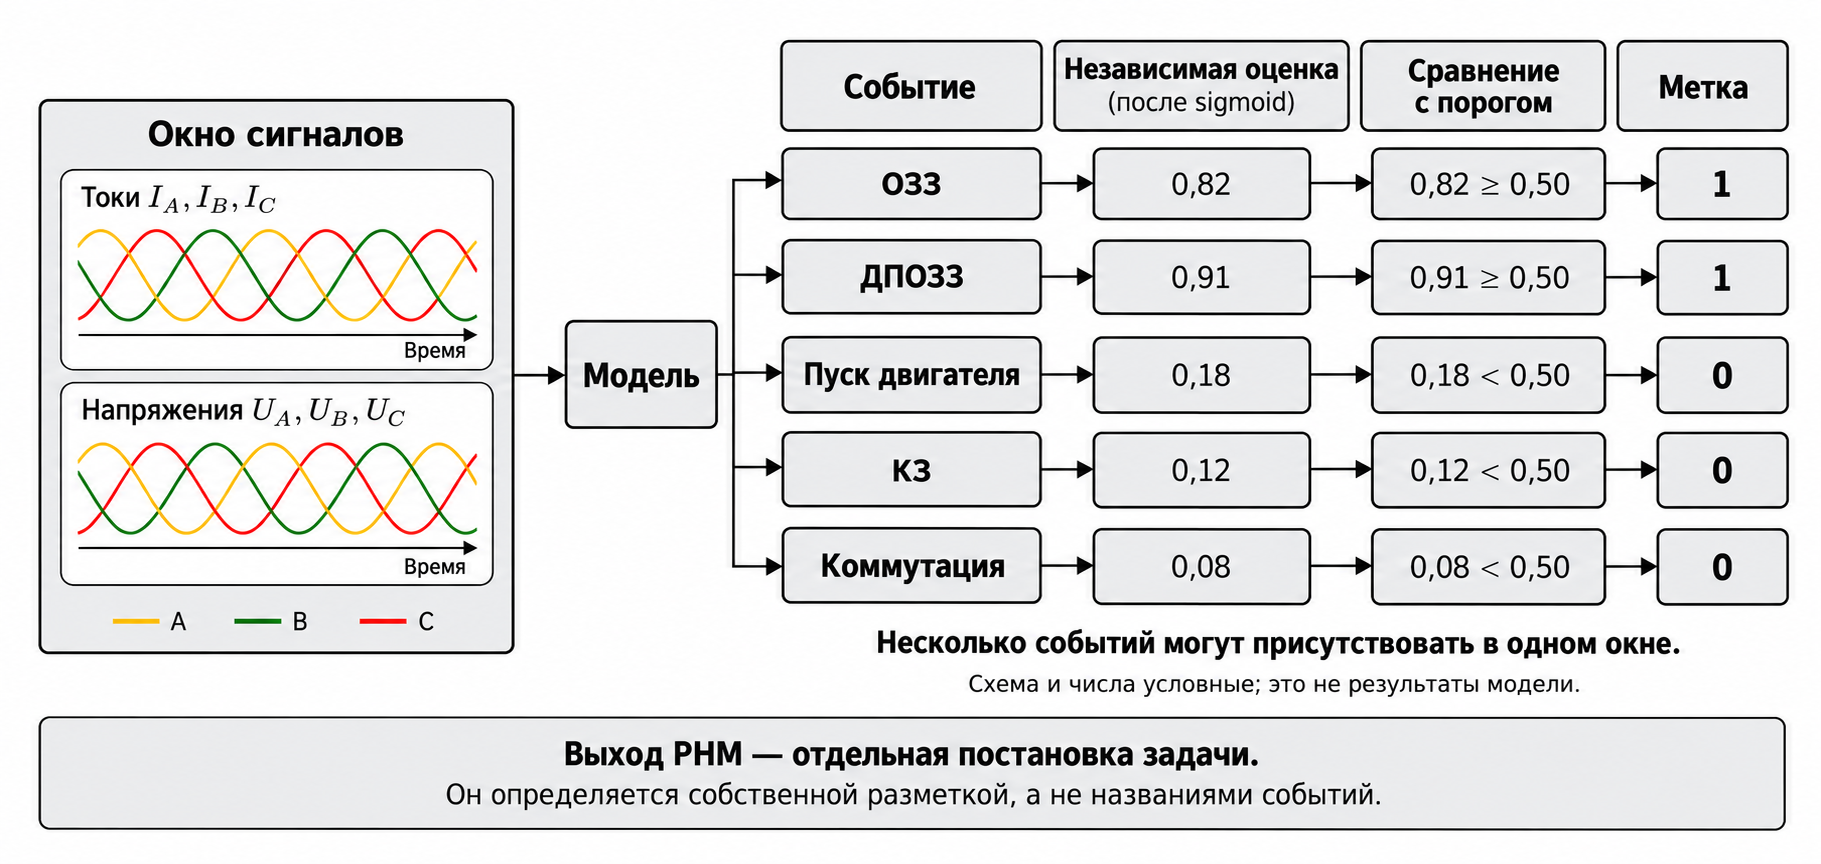
\includegraphics[width=\textwidth]{ch04_output_decision_candidate.png}
    \caption{Оценки событий и получение меток при сравнении с порогом.
    Условный пример, не результат испытания модели}
    \label{fig:ch4_output_decision}
\end{figure}

Такое различие существенно для переходных процессов. В одном
фрагменте могут присутствовать ОЗЗ, последующее КЗ и коммутация.
Метка всего окна, метка последнего отсчёта и наличие события
хотя бы в части окна задают различные обучающие задачи.
Даже одинаковая архитектура будет обучаться разному поведению,
если изменится это правило. Устройство сети далее рассматривается
отдельно от конкретного правила разметки и численных результатов.

\subsection{Полносвязная модель SimpleMLP}
\label{sec:ch4_simplemlp}


Для сопоставления способов обработки рассматриваются полносвязная,
свёрточная и остаточная архитектуры. В модели SimpleMLP входное
окно преобразуется в вектор признаков, который поступает
в последовательность полносвязных слоёв. 
\iffalse
(Примечание автора: Есть мысли о том, чтобы картинки тут привести поясняющие схему, 
если у меня в оригинальных работах есть. Убрать потом это, в случае чего будет не сложно, 
а пока что хочу максимально подробно переписывать статьи. 
Кстати, об этом опять же можешь сделать пометку, она будет полезна для будущего текста
Причём... Можно подумать о том, чтобы нарисовать какую-то другую картинку поясняющую, как я делал в будущих работах, 
я думаю современные ИИ модели могут помочь сдлеать её тут, надо будет только инструкцию хорошую написать для картинки,
если тебе сложно. И да, лучше через инструкцию сделать это, а не тебе самой выдумывать, причём я хочу тут иснтрукцию
поясняющую проблему для энергетики, где у меня подаются и ТОКИ и НАПРЯЖЕНИЯ и по времени распределены и они путаются.
Да, давай попробуем через картинки такие новые.
Хмм... В статье есть картинки, но они довольно сложны, и не факт, что отражают физическую проблему) **[AA040: закрыто автором; сохранено в истории]**.
(Примечание автора: Считаю задачу закрытой, если что-то нужно всё же оставить - то сделай отдельным примечанием и там, где оно нужно по локации)
\fi
\authorreviewnote{AA040}
\iffalse
(Примечание автора: И да, ещё раз отмечу, давай побольше текста пока что из оригинальных работ писать сюда.
Да, не весь и не всё, но важное, люди из энергетики многое базовое могу не понимать.) **[AA041: закрыто автором; сохранено в истории]**.
(Примечание автора: Считаю закрытой)
\fi
\authorreviewnote{AA041}
Взаимосвязи компонентов определяются обучаемыми весами. Порядок отсчётов сохраняется
в положении элементов вектора, однако локальная временная структура
не задаётся специальным механизмом архитектуры. Такая модель
служит исходным вариантом для сравнения более структурированных
способов обработки.

На рисунке~\ref{fig:ch4_mlp_flow} показана последовательность
обработки в SimpleMLP. Операция развёртывания не вычисляет новых
физических признаков. Она размещает компоненты матрицы $X$
в одном векторе $\boldsymbol{x}$ длины $CT$. Значение в определённой
позиции вектора связано с конкретным каналом и положением в окне.
При изменении длины окна меняется размер входа первого
полносвязного слоя.

\iffalse
(Примечание автора: Урезал картинку, если нужно старое из неё - добавь где-то в текст. Находится в папке "_Устаревшее для памяти") **[AA076: рассмотрено 22.10; ожидает проверки]**
(Примечание автора: Закрывай задачу.)
\fi
\authorreviewnote{AA076}

\begin{figure}[htbp]
    \centering
    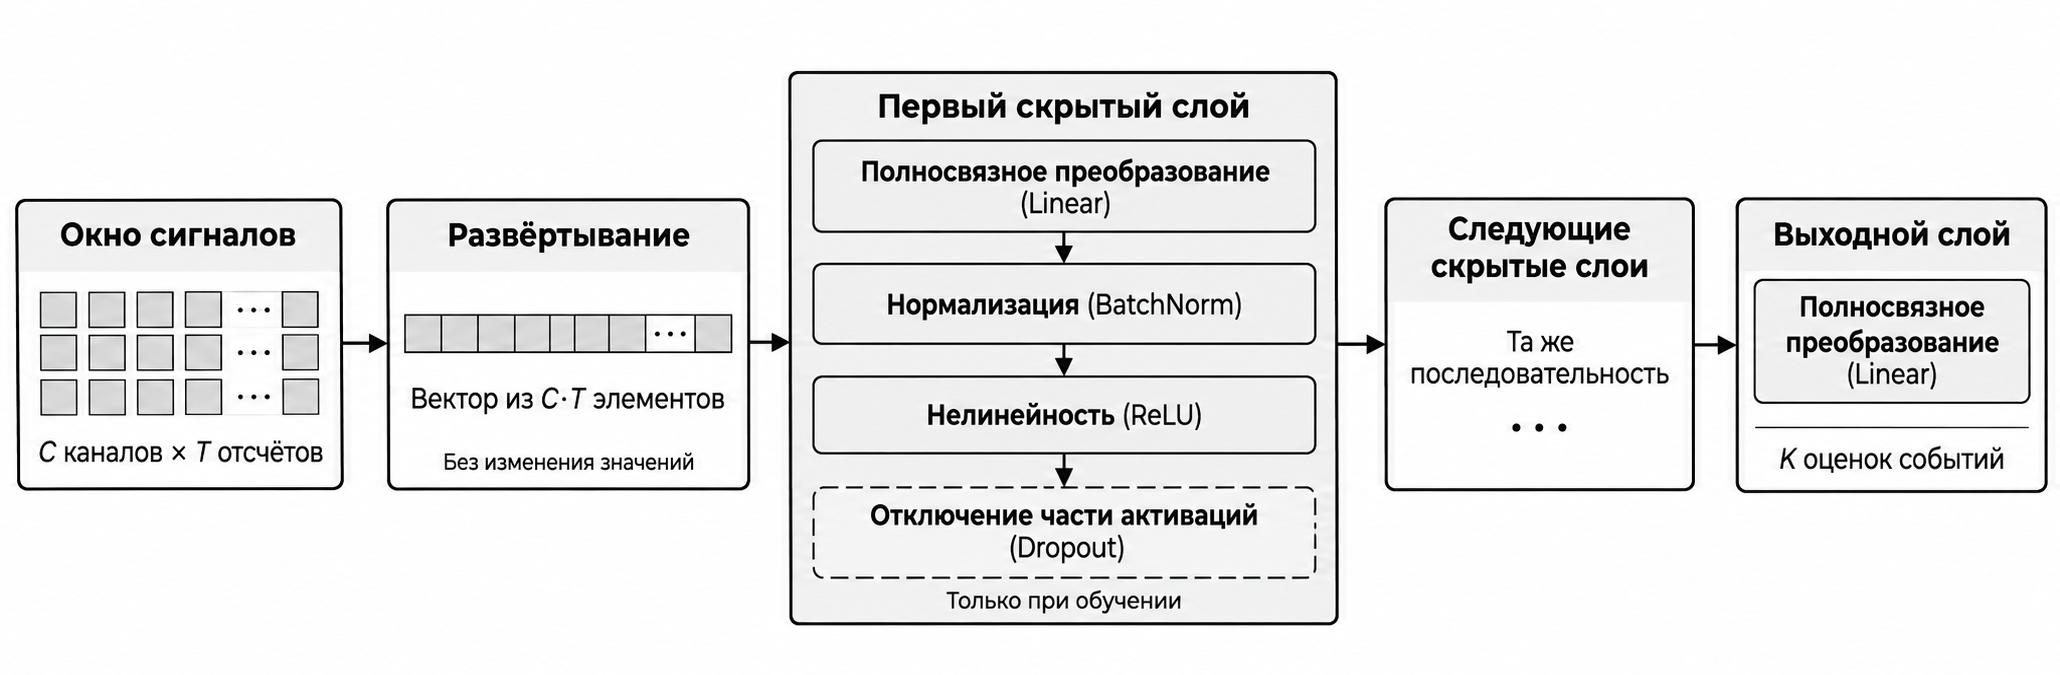
\includegraphics[width=\textwidth]{physkan_mlp.png}
    \caption{Последовательность обработки в SimpleMLP. Показан вариант
    с нормализацией и отключением части активаций при обучении}
    \label{fig:ch4_mlp_flow}
\end{figure}


\iffalse
(Примечание автора: Добавил вот этот файл, используй теперь его «physkan_mlp.png», аналогично сделаю для следующих картинок.) **[AA049: закрыто автором; сохранено в истории]**
(Примечание автора: Да, добавлено, всё есть, закрываем)
\fi
\authorreviewnote{AA049}


Полносвязное преобразование слоя имеет вид
\begin{equation}
    h_j=\rho\left(\sum_{i=1}^{n}w_{ji}x_i+b_j\right),
    \label{eq:ch4_mlp_layer}
\end{equation}
где $w_{ji}$ являются весами связей, $b_j$ смещением,
а $\rho$ функцией активации. В реализации SimpleMLP используется
$\operatorname{ReLU}(x)=\max(0,x)$. Между линейным преобразованием
и ReLU может выполняться нормализация BatchNorm (BN).
При обучении после активации применяется Dropout,
который случайно отключает часть компонент согласно заданной
вероятности. Это средство регулирования обучения,
а не моделирование отказа конкретного измерительного канала.
При оценке обученной модели случайное отключение прекращается.

Выход первого слоя поступает в следующий слой в качестве
нового вектора. Такая последовательность формирует составное
нелинейное преобразование. Последний линейный слой связывает
скрытые признаки с оценками событий. Для слоя с $n$ входами
и $m$ выходами число весов и смещений равно $(n+1)m$.
Например, переход от условного входа из 192 компонент
к 64 выходам содержит 12\,352 таких параметра.
Параметры нормализации, если она включена, учитываются отдельно.

Полносвязная модель допускает взаимодействие любых входных
компонент уже в первом слое. При этом один и тот же локальный
процесс, смещённый внутри окна, попадает на другие позиции
и связывается с другим набором весов. Сеть может научиться
учитывать такие смещения по данным, но общая для всех положений
операция обработки не задана её структурой. Это объясняет,
зачем наряду с SimpleMLP исследуются модели, непосредственно
использующие локальные связи вдоль окна.

\subsection{Свёрточная модель SimpleCNN}
\label{sec:ch4_simplecnn}

В модели SimpleCNN одномерные свёртки обрабатывают соседние отсчёты
и используют общие коэффициенты в разных положениях окна.
Это позволяет выделять локальные изменения формы сигнала
одним набором обучаемых фильтров. Последовательность слоёв
объединяет локальные признаки в описание рассматриваемого процесса.
Подобно привычной в РЗА фильтрации при выделении гармоник,
свёртка формирует взвешенную сумму отсчётов. При преобразовании
Фурье коэффициенты задаются синусоидальными функциями выбранных
частот. Здесь коэффициенты подбираются при обучении и могут
выделять фронты, искажения и другие характерные формы сигнала.
Физический смысл каждого фильтра заранее не фиксируется,
поэтому его связь с конкретным измерительным признаком
требует отдельного анализа.

\iffalse
(Примечание автора: Можно добавить, что по своей сути чем-то близко к Фурье обработки сигналов, что типично для энергетики.
Но может выделять совсем разные патерны) **[AA050: закрыто автором; сохранено в истории]**
(Примечание автора: Да, закрываем примечание.)
\fi
\authorreviewnote{AA050}


Свёрточный слой последовательно рассматривает локальные участки
входа. Для каждого выходного канала формируется отклик
по всем входным каналам и позициям внутри ядра. При единичном
шаге и без разрежения ядра это преобразование можно записать
в виде
\begin{equation}
    v_o(t)=b_o+\sum_{c=1}^{C}\sum_{r=0}^{k-1}
        w_{ocr}X_c(t+r-p),
    \label{eq:ch4_conv_layer}
\end{equation}
где $k$ задаёт размер ядра, а $p$ величину дополнения
на границах. В практической реализации также выбирается шаг,
с которым ядро перемещается вдоль обрабатываемой оси.
Одинаковые коэффициенты $w_{ocr}$ используются в разных
положениях окна.

При шести входных каналах, 16 выходных каналах и ядре длины три
свёртка содержит $16(6\cdot3+1)=304$ веса и смещения.
Это условный пример устройства одного слоя. Он не является
сравнением итоговых размеров CNN и MLP, поскольку их последующие
слои и число извлекаемых признаков могут различаться.
Для свёртки с неизменным ядром число весов не зависит
от длины входного окна, хотя объём вычислений зависит от неё.

\begin{figure}[htbp]
    \centering
    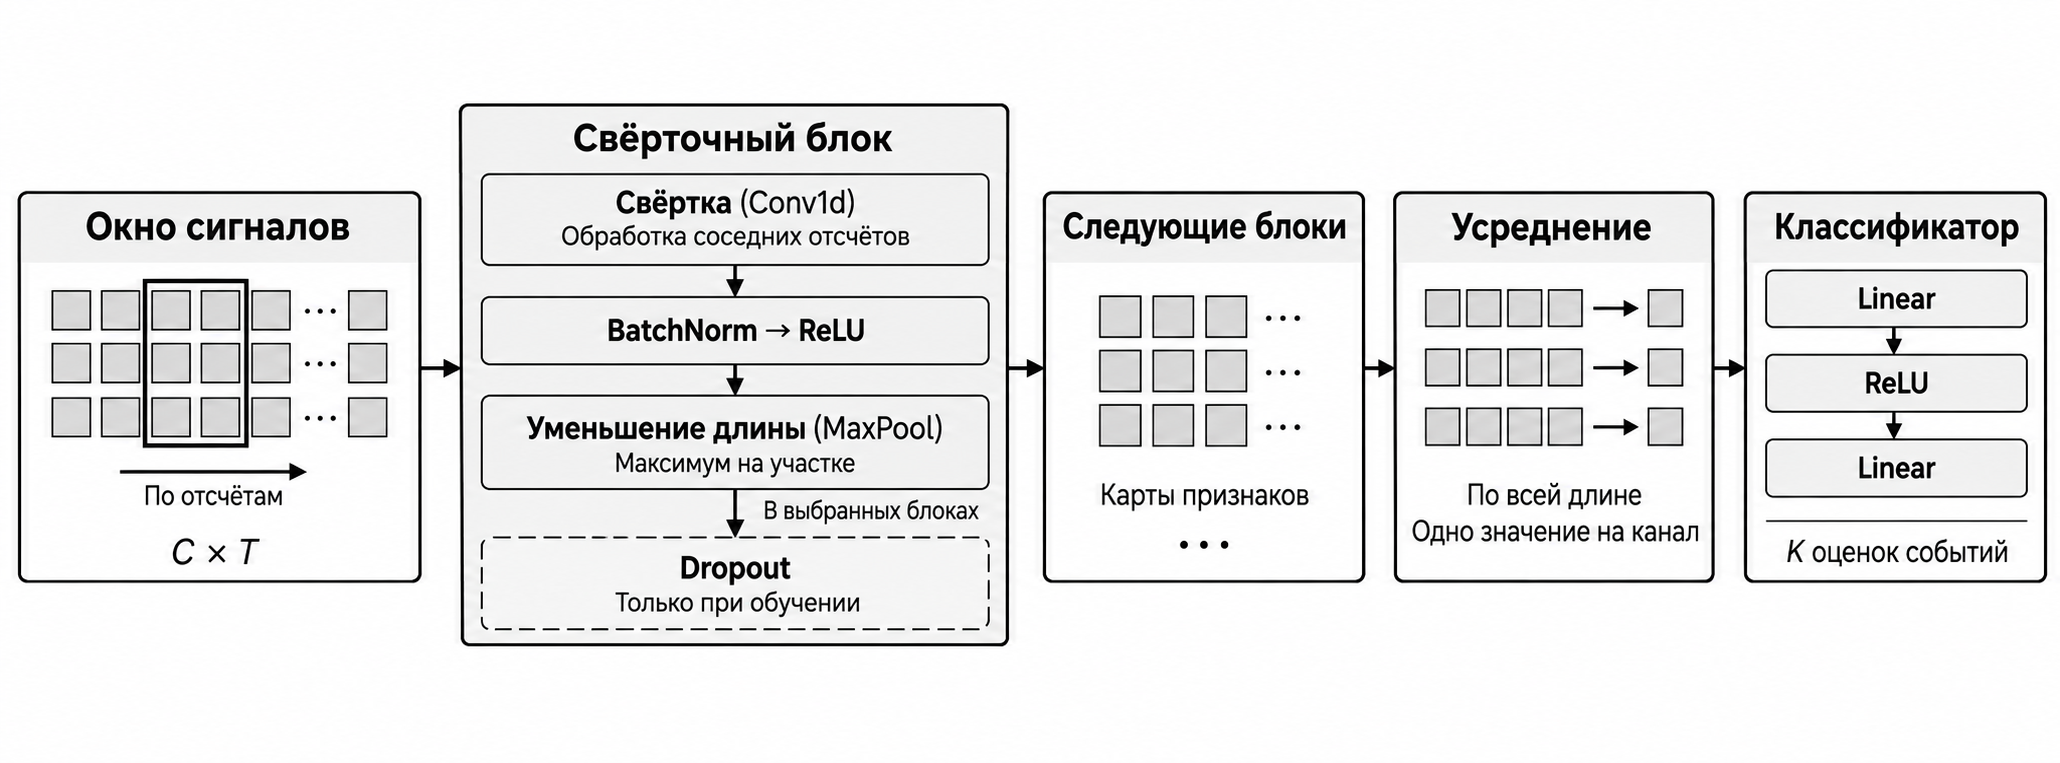
\includegraphics[width=\textwidth]{physkan_cnn.png}
    \caption{Обработка окна в SimpleCNN. Свёрточные блоки выделяют
    локальные признаки, затем выполняется усреднение вдоль окна}
    \label{fig:ch4_cnn_flow}
\end{figure}

В рассматриваемой SimpleCNN за свёрткой могут следовать
BatchNorm и ReLU. После выбранных блоков применяется MaxPool,
который оставляет наибольший отклик в небольшом участке
обрабатываемой оси. Длина последовательности при этом
уменьшается. Если участок уже короче необходимого размера,
защитный вариант операции пропускает это уменьшение.
Dropout используется при обучении после обработки блока.

Следующий свёрточный слой получает карты признаков предыдущего,
а не исходные каналы тока и напряжения. Его отклик объединяет
информацию из нескольких локальных участков исходного окна.
Так последовательно расширяется область входа, которая может
влиять на один внутренний признак. Обученные карты могут
отражать фронты, колебания или сочетания сигналов, однако
содержание каждого отклика определяется обучением.

В конце SimpleCNN выполняется адаптивное усреднение по всей
оставшейся оси. Каждый канал даёт одно значение независимо
от текущей длины карты. Полученный вектор поступает в две
полносвязные ступени классификатора с промежуточной ReLU,
как показано на рисунке~\ref{fig:ch4_cnn_flow}.
Такой выход описывает окно в целом. Само усреднение
не определяет точное положение границы события,
поэтому локализация должна задаваться отдельной постановкой
или способом применения модели к последовательности окон.

\subsection{Остаточная модель ResNet1D}
\label{sec:ch4_resnet}

В модели ResNet1D применяются остаточные связи. Эта модель
используется для проверки более глубокой обработки сигналов
по сравнению с исходной MLP и простой свёрточной сетью.
Сопоставление позволяет оценивать влияние увеличения глубины
при сохранении обходного пути передачи признаков.
Выход блока
суммируется с его входом после необходимого согласования
размерностей. Это сохраняет путь передачи исходной информации
и позволяет обучать последовательность преобразований.
Увеличение глубины и числа каналов меняет объём вычислений
и количество параметров. Поэтому архитектура оценивается
совместно с её конкретной конфигурацией и представлением входа.
Само название модели не определяет ни качество распознавания,
ни возможность её применения в микропроцессорном устройстве.

\iffalse
(Примечание автора: Ну да, как-то очень кратко... Мне-то понятно, но я всё это и написал ранее.) **[AA042: закрыто автором; сохранено в истории]**
(Примечание автора: Всё нормально, можно закрыть.)
\fi
\authorreviewnote{AA042}

Основной элемент ResNet1D объединяет два пути передачи данных,
показанные на рисунке~\ref{fig:ch4_residual_flow}.
В основном пути выполняются свёртка, нормализация и ReLU,
затем вторая свёртка и нормализация. Обозначим полученное
преобразование $F(\boldsymbol{x})$. По обходному пути передаётся
сам вход либо его проекция $P(\boldsymbol{x})$,
согласующая число каналов и длину последовательности.
После суммирования применяется ReLU.
\begin{equation}
    \boldsymbol{y}=\operatorname{ReLU}
       \bigl(F(\boldsymbol{x})+P(\boldsymbol{x})\bigr).
    \label{eq:ch4_residual_block}
\end{equation}
При совпадении размерностей $P$ является тождественным
преобразованием. В рассматриваемой реализации для согласования
используются свёртка с ядром длины один и нормализация.

\begin{figure}[htbp]
    \centering
    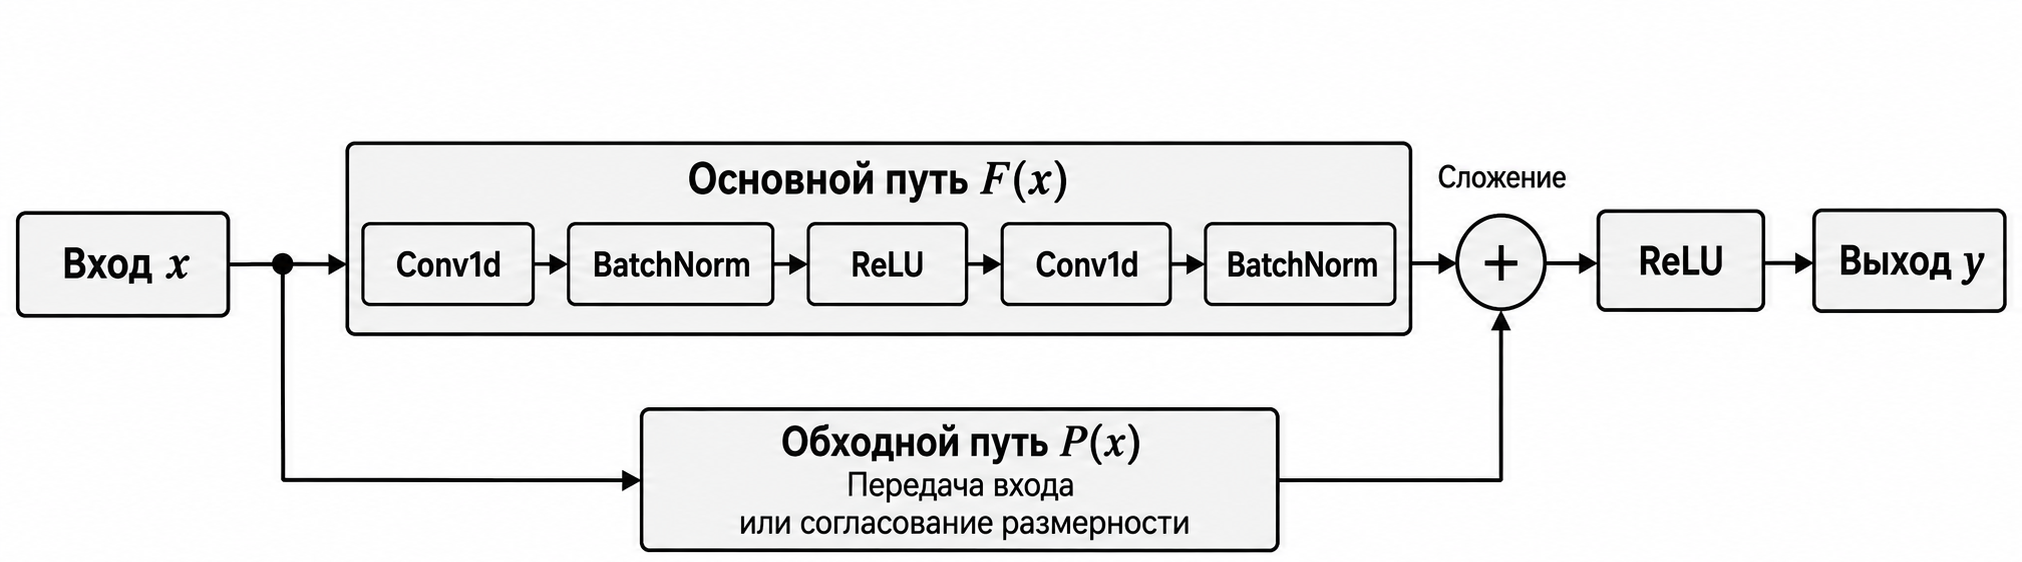
\includegraphics[width=\textwidth]{physkan_residual.png}
    \caption{Остаточный блок ResNet1D. Обходной путь передаёт вход
    непосредственно или согласует его размерность перед суммированием}
    \label{fig:ch4_residual_flow}
\end{figure}

Обходной путь позволяет сохранить информацию, которая уже
представлена на входе блока. Основной путь обучается её
преобразованию, а сумма объединяет обе составляющие.
При обучении производная проходит и через основной путь,
и через обходной. Это структурное свойство помогает обучению
последовательности блоков, но не задаёт физическую верность
полученного признака.

В рассматриваемой ResNet1D перед остаточными ступенями
находятся начальная свёртка, нормализация, ReLU и уменьшение
длины последовательности. Далее следуют четыре ступени,
в которых число каналов относительно начального значения
последовательно изменяется в отношении $1:2:4:8$.
Количество блоков внутри ступеней определяется конфигурацией.
Последние карты усредняются вдоль обрабатываемой оси,
после чего линейный классификатор формирует оценки событий.

Такая организация даёт возможность наращивать глубину
обработки. Вместе с тем увеличение числа каналов и блоков
меняет память и количество операций. Сравнение с другими
моделями требует указания конкретной конфигурации,
а не только названия ResNet1D. Оценка на зарегистрированных
режимах должна показать, какие ошибки изменяются при таком
усложнении и какой вычислительный объём для этого требуется.


\iffalse
(Примечание автора: Надо бы что-то добавить о том, чем она лучше других, а то зачем мы её вообще внедряли?) **[AA051: закрыто автором; сохранено в истории]**
(Примечание автора: Да, всё сдеално, закрывай.)
\fi
\authorreviewnote{AA051}


\subsection{KAN-слои и модели SimpleKAN и ConvKAN}
\label{sec:ch4_kan}

В сетях Колмогорова--Арнольда обучаемые одномерные функции
располагаются на связях между компонентами соседних слоёв.
В отличие от полносвязного слоя с фиксированной функцией активации,
обучение изменяет форму этих зависимостей. В исходных SimpleKAN и ConvKAN
используются функции на основе B-сплайнов.\footnote{Liu Z. et al.
KAN: Kolmogorov--Arnold Networks. 2025.
\url{https://arxiv.org/abs/2404.19756v5}.}
Для входного вектора $\boldsymbol{x}$ преобразование слоя
можно записать в виде
\begin{equation}
    y_j = \sum_{i=1}^{n} f_{ji}(x_i),
    \label{eq:ch4_kan_layer}
\end{equation}
где $f_{ji}$ обозначает обучаемую функцию на соответствующей связи.
Состав и ширина последовательности слоёв задают сложность модели.

На рисунке~\ref{fig:ch4_kan_flow} показан условный слой
с двумя входами и двумя выходами. Каждый вход передаётся
через свою обучаемую функцию к каждому выходу,
а результаты суммируются. Функции разных связей
не обязаны совпадать. Таким образом, изменение формы
зависимости на одной связи не означает такое же изменение
на остальных связях.

\iffalse
(Примечание автора: Урезал картинку, если нужно старое из неё - добавь где-то в текст. Находится в папке "_Устаревшее для памяти") **[AA076: рассмотрено 22.10; ожидает проверки]**
(Примечание автора: Закрывай задачу.)
\fi

\begin{figure}[htbp]
    \centering
    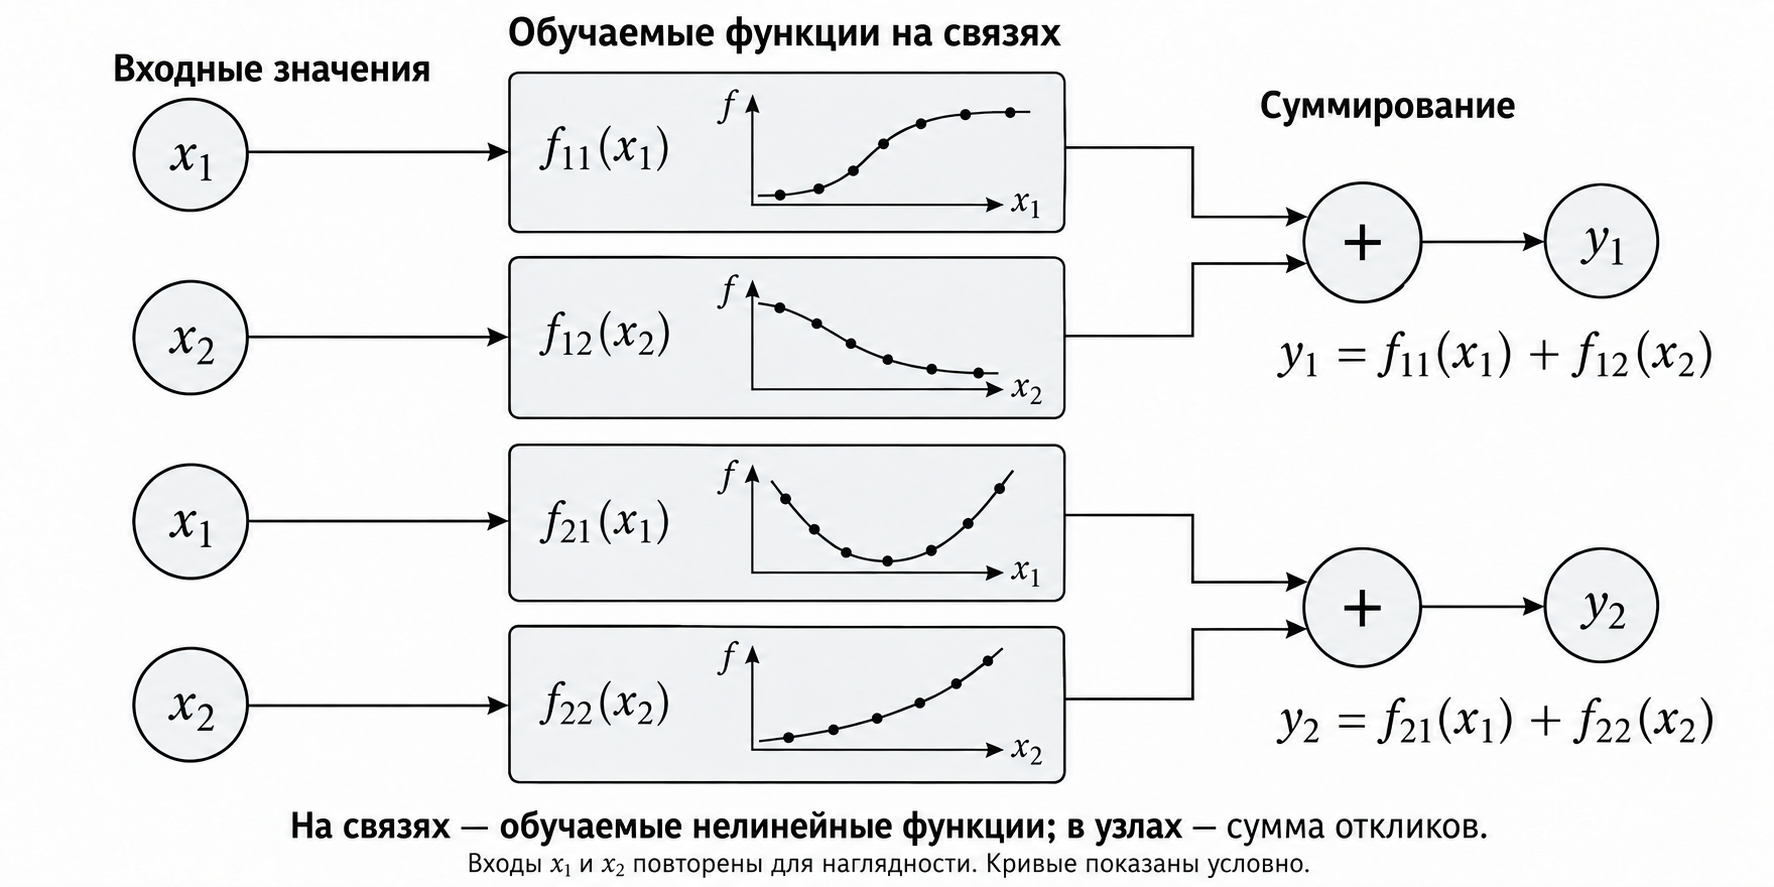
\includegraphics[width=\textwidth]{physkan_kan_edge.png}
    \caption{Принцип KAN-слоя на условном примере двух входов
    и двух выходов. Схема не изображает обученные функции конкретной модели}
    \label{fig:ch4_kan_flow}
\end{figure}

В используемом KANLinear функция связи содержит базовую
нелинейную часть и сплайновую составляющую. Её можно представить
как
\begin{equation}
    f_{ji}(x)=a_{ji}\psi(x)+\sum_{q=1}^{Q}c_{jiq}B_q(x),
    \label{eq:ch4_kan_spline}
\end{equation}
где $\psi$ обозначает базовую функцию активации,
$B_q$ функции сплайнового базиса,
а $a_{ji}$ и $c_{jiq}$ обучаемые коэффициенты.
В рассматриваемом варианте базовой функцией служит SiLU,
$\psi(x)=x/(1+e^{-x})$. Масштабы сплайновой части
могут учитываться в коэффициентах $c_{jiq}$.

Для нелинейных характеристик измерительных органов
важна возможность менять не только наклон линейной зависимости,
но и форму её отдельных участков. Например, реакция на изменение
тока может быть слабой до определённой области и значительно
более выраженной после её достижения. Другая зависимость
может иметь область малой чувствительности или ограничение
выходного отклика. Обучаемая функция на связи позволяет
представлять такие различия непосредственно своей формой.
Этот пример объясняет математическую возможность,
а не подтверждённую характеристику обученного реле.

В MLP нелинейность формируется сочетанием линейных
преобразований и фиксированных активаций.
В KAN изменяется и сама одномерная зависимость
между выбранными компонентами соседних слоёв.
Это даёт иной способ представления сильно нелинейной
связи. Для задачи анализа осциллограмм представляет интерес
возможность исследовать такую функцию отдельно
и установить, в каких областях признака меняется её отклик.
При этом MLP также может представлять нелинейные зависимости,
поэтому преимущество конкретного варианта устанавливается
в экспериментальном сравнении.

Одномерная функция на связи не заменяет взаимодействие
нескольких физических величин. Например, направление мощности
определяется не только амплитудой тока, но и напряжением
и фазовым соотношением. Взаимодействия между компонентами
возникают при последовательной обработке в слоях.
В физически мотивированных вариантах произведения,
отношения и фазовое управление дополнительно задают
структуру таких взаимодействий. Тем самым обучаемая
нелинейность KAN и включение физической арифметики
решают связанные, но различные задачи.

Сплайновый базис задаётся сеткой узлов и выбранным порядком.
Каждая базисная функция действует на ограниченной области
входной оси. Обучение изменяет коэффициенты их сочетания,
формируя общую зависимость $f_{ji}$. Плотность узлов
и порядок сплайна определяют возможности представления
функции и число необходимых коэффициентов.
Поэтому на одну связь KAN может приходиться больше одного
обучаемого параметра. Малое число нейронов само по себе
не означает малого общего числа параметров.


\iffalse
(Примечание автора:Посмотрим, как подробно об этом было в статье, кажется, что местами начала закапываться в подробности математики у нас. Хотя… Про сплайновые подходы может быть и полезно. Согласен) **[AA052: закрыто автором; сохранено в истории]**
(Примечание автора: Ок, закрываем)
\fi
\authorreviewnote{AA052}



\iffalse
(Примечание автора: Потом, наверное про модельку КАН – надо бы какую-то картинку? Может из статьи что-то взять поясняющее? Или опиши текстом, что хочешь? Или может в статье есть… Хотя… Хотя там в отрисовке самих моделей. В общем – надо бы что-то поясняющее про КАН подход и зачем такое хорошо, пожалуй, какой-то картинкой к этому тексту.) **[AA053: закрыто автором; сохранено в истории]**
(Примечание автора: Закрываем.)
\fi
\authorreviewnote{AA053}



\iffalse
(Примечание автора: И надо ли тут описывать модели, если оно идёт прям следом?. Да и разделы чуть другие получаются, сперва базовые модели по отдельности, потом идёт какое-то Описание КАН, не понятно к чему, а потом ещё, быть может, вставим Трансформерные модели, кстати, а здесь ли их вообще вставлять? Или когда-то позже, ведь статьи это совсем разные, но это к более глоабльному вопросу, который ставлю по всему разделу 4… А конкретно в этой точке – вопрос в том, что под КАН идёт отдельный номер описания, но не описывает конкретную модель) **[AA054: закрыто автором; сохранено в истории]**
(Примечание автора: Закрываем, уже устарело замечание.)
\fi
\authorreviewnote{AA054}



\iffalse
(Примечание автора: Хотя ошибся в комментарии, да, описание SimpleKAN, ConvKAN , есть смысл оставить, ибо это краткая вставка, а дальше про физически модели речь. Извиняюсь, ошибка моя, коммент тот не удалял, может там что-то другое имеет значение) **[AA055: закрыто автором; сохранено в истории]**
(Примечание автора: Закрываем, устарело.)
\fi
\authorreviewnote{AA055}



\iffalse
(Примечание автора: ошибся, поясняющая КАН картинка в общем-то есть, и я её улушчил, это "Рис. 4.4: Принцип KAN-слоя") **[AA056: закрыто автором; сохранено в истории]**
(Примечание автора: Закрываем, устарело.)
\fi
\authorreviewnote{AA056}


В трансформерном варианте используется реализация FastKAN.
В ней обучаемая зависимость формируется с помощью гауссовых
радиальных базисных функций и базового преобразования SiLU.
Это другой способ задания функций на связях, поэтому описание
B-сплайнов и их порядка не переносится на FastKAN буквально.
Общий принцип обучения одномерных зависимостей при этом сохраняется.
В расширенном исследовании признакового пространства
для SimpleKAN и ConvKAN используется ещё один вариант базиса,
полиномы Чебышёва третьей степени. Он также задаёт обучаемые
функции на связях. Эти реализации различаются способом
вычисления функций и не отождествляются только по названию KAN.
Выбор FastKAN связан с уменьшением затрат на вычисление
обучаемых функций при обработке последовательности окон.
Гауссовы базисные функции упрощают эту часть расчёта по сравнению
с непосредственным вычислением B-сплайнов. Время работы всей
модели при этом определяется также её размерами и остальными слоями.


\iffalse
(Примечание автора: Чуть чуть пояснить, почему выбрали её. Не помню точно, может где-то описано, проводил отдельный этап исследований, а кратко вроде бы - сей вариант наиболее быстрый.) **[AA072: закрыто автором; сохранено в истории]**
(Примечание автора: Да, вопрос закрыт)
\fi
\authorreviewnote{AA072}

Модель SimpleKAN использует такие преобразования для обработки
входного вектора. Модель ConvKAN сочетает свёрточную обработку
с нелинейными преобразованиями на основе KAN. Временная структура
входа при этом используется для выделения локальных признаков,
а форма обучаемых функций может быть рассмотрена отдельно.

SimpleKAN развёртывает многоканальный вход в вектор,
как и SimpleMLP. Затем он проходит последовательность KANLinear
с заданными размерами скрытых слоёв. В этих слоях уже содержится
нелинейное преобразование связей, поэтому они не сводятся
к замене одной ReLU другой фиксированной функцией.
Последний KANLinear формирует требуемое число выходных оценок.
Изменение длины развёрнутого входа меняет число связей
первого слоя и должно учитываться при сравнении моделей.

В ConvKAN операция выполняется над локальными участками.
Для каждого положения из всех каналов извлекается участок
длины $k$ и развёртывается в вектор длины $Ck$.
Один KANLinear преобразует каждый такой вектор
в набор выходных каналов. Затем результаты возвращаются
в структуру карт признаков вдоль обрабатываемой оси.
Параметры преобразования общие для разных положений участка.

Таким образом, ConvKAN сохраняет локальную обработку
и повторное использование одного преобразования,
характерные для свёрточной сети. При этом зависимость
выхода от элементов локального участка задаётся
обучаемыми функциями на связях. В рассматриваемой реализации
после KAN-свёрток применяются нормализация,
уменьшение длины выбранных карт и Dropout при обучении.
Итоговое усреднение формирует вектор для двух KANLinear
классификатора.

Возможность построить график функции на связи полезна для анализа
модели. Однако наличие такого графика само по себе не устанавливает
электротехнический смысл соответствующего признака. Внутренние
переменные могут представлять обученные комбинации сигналов.
Для содержательного объяснения необходима связь этих переменных
с входными величинами и поведением модели на известных режимах.

\iffalse
(Примечание автора: Из текста не очень понятно, чем это лучше предыдущего?
Я закладывал во многом то, чтобы могли возникать сильно нелинейные связи например от тока и т.д. Ну и да, побольше бы описания…) **[AA043: закрыто автором; сохранено в истории]**
(Примечание автора: Ок, закрываем)
\fi
\authorreviewnote{AA043}

\subsection{Вещественные физические операции}
\label{sec:ch4_real_ops}

В архитектуре PhysicsKAN введены операции попарного умножения
и деления входных каналов. При согласованном расположении токов
и напряжений эти операции формируют признаки, связанные
с их произведениями и отношениями. Для мгновенных значений
однофазных сигналов произведение $u(t)i(t)$ соответствует
мгновенной мощности. Отношение $i(t)/u(t)$ характеризует
взаимосвязь сигналов, но при переходном процессе не становится
автоматически оценкой постоянной проводимости элемента сети.

Для вещественного блока вход упорядочивается так,
чтобы две равные группы каналов содержали сопоставляемые
величины. Обозначим их $\boldsymbol{x}_I$
и $\boldsymbol{x}_U$. При правильном составе пар
умножение формирует $\boldsymbol{x}_I\odot\boldsymbol{x}_U$,
а деление отношение первой группы ко второй.
Сам арифметический блок не распознаёт названия каналов
и не проверяет их соответствие одной фазе.
Поэтому порядок подготовки данных входит в определение модели.

На рисунке~\ref{fig:ch4_physics_stem} показаны три пути передачи
информации. При $C$ входных каналах каждая арифметическая ветвь
формирует $C/2$ новых каналов. Они объединяются с $C$ исходными,
давая $2C$ каналов для дальнейшей обработки.
Например, три канала токов и три соответствующих канала
напряжений дают три произведения и три отношения.
Вместе с шестью исходными сигналами получается 12 каналов.
Такой подсчёт характеризует рассматриваемый вещественный блок,
а не размер произвольного гармонического представления.

\iffalse
(Примечание автора: Урезал картинку, если нужно старое из неё - добавь где-то в текст. Находится в папке "_Устаревшее для памяти") **[AA076: рассмотрено 22.10; ожидает проверки]**
(Примечание автора: Закрывай задачу.)
\fi

\begin{figure}[htbp]
    \centering
    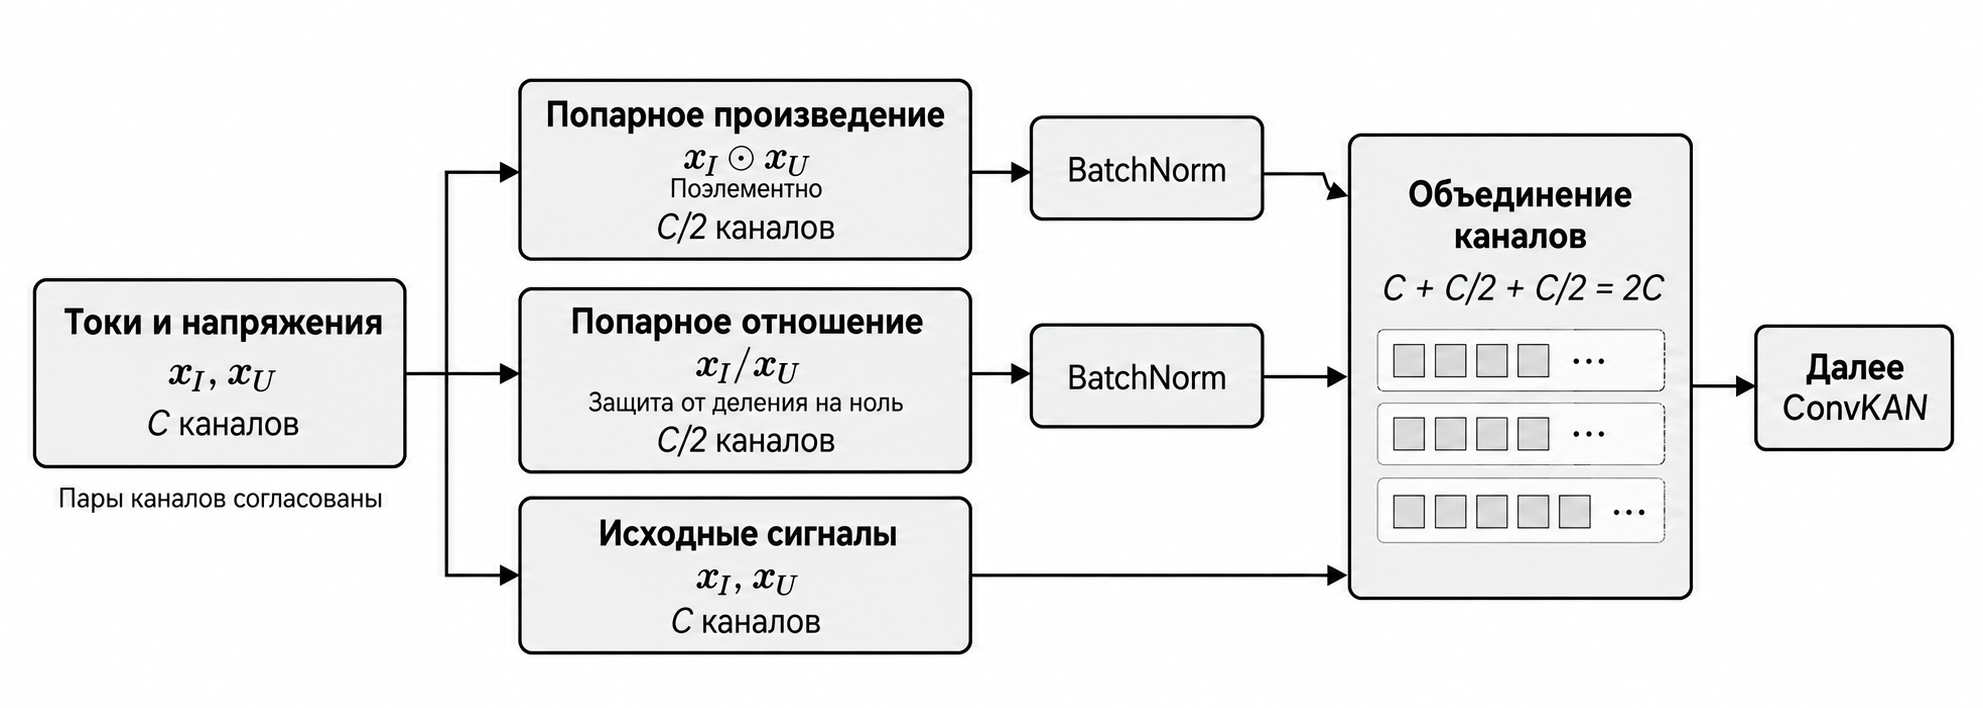
\includegraphics[width=\textwidth]{physkan_arithmetic_stem.png}
    \caption{Входной физический блок PhysicsKAN. Исходные каналы
    дополняются нормализованными произведениями и отношениями}
    \label{fig:ch4_physics_stem}
\end{figure}

При делении требуется учитывать малые значения знаменателя.
Для вещественного сигнала используется подстановка значений
порядка выбранного малого порога. Она уменьшает чувствительность
отношения к знаменателю вблизи нуля, но полученный признак
всё ещё может принимать большие значения. Поэтому
вычислительное ограничение и физическая пригодность признака
рассматриваются отдельно.

Пусть $d$ является вещественным знаменателем,
а $\varepsilon>0$ выбранной малой величиной.
Если $|d|\geq\varepsilon$, деление выполняется с исходным
знаменателем. В области $|d|<\varepsilon$ программная
подстановка использует знак $d$ с небольшим положительным
сдвигом. При точном нуле получается положительное значение.
Поэтому это правило отличается от строгого сохранения знака
в сколь угодно малой окрестности нуля. Параметры ограничения
влияют на признаки и производные в этой области.

Входные токи и напряжения предварительно приводятся
к принятому масштабу. Поэтому арифметический выход сети
может быть относительным признаком, а не величиной
в ваттах или сименсах. Для восстановления физических единиц
необходимо учитывать коэффициенты подготовки обоих каналов.
В частности, разные коэффициенты масштабирования числителя
и знаменателя изменяют масштаб их отношения.

Сформированные каналы проходят нормализацию и объединяются
с исходными каналами. Последующая обработка сохраняет доступ
и к исходным сигналам, и к результатам физических операций.
Обучаемая часть определяет, какие из них существенны
для рассматриваемой задачи. Арифметические операции включены
в общий граф вычислений, через который проходит обучение.

В рассматриваемом базовом варианте физические операции выполняются
при входной обработке, перед последовательностью KAN-слоёв.
Их применение к признакам на последующих уровнях представляет
другое архитектурное развитие. После обучаемых преобразований
скрытые каналы могут утрачивать непосредственный смысл токов
и напряжений. Поэтому произведения и отношения таких каналов
нуждаются в собственной интерпретации.

Физический входной блок не имеет такого же состава
обучаемых весов, как полносвязный слой. Основные произведения
и отношения определены непосредственно операциями.
При обучении меняются последующие преобразования
и параметры нормализации. Производная выходного результата
передаётся через арифметические ветви, связывая их
с общей процедурой обучения.

Для произведения производная по одному сомножителю равна
другому. Для отношения вне области ограничения знаменателя
она содержит величины $1/u$ и $-i/u^2$.
Это объясняет, почему малое напряжение влияет не только
на величину дополнительного признака, но и на чувствительность
вычислений при обучении. Ограничение знаменателя
и нормализация выполняют разные задачи и должны
рассматриваться совместно.

В варианте с временной обработкой объединённый набор поступает
в ConvKAN. При коротком входном представлении возможна
обработка развёрнутого набора через SimpleKAN.
Обе организации сохраняют одинаковую идею добавления
арифметических признаков, но по-разному используют ось
положений входа. Выбор между ними относится к конфигурации
модели и должен быть указан в экспериментальном сравнении.

\subsection{Комплексные признаки и фазовые соотношения}
\label{sec:ch4_complex_ops}

При использовании гармонических составляющих существенны
не только амплитуды, но и фазовые соотношения сигналов.
В архитектуре cPhysicsKAN комплексные величины представлены
парами амплитуды и фазы. Порядок каналов согласован с этим
представлением, а операции выполняются одновременно
над обеими компонентами каждой пары.

Для величин $z_1=A_1e^{\mathrm{j}\varphi_1}$
и $z_2=A_2e^{\mathrm{j}\varphi_2}$ произведение и отношение
имеют вид
\begin{equation}
\begin{aligned}
    z_1z_2 &= A_1A_2e^{\mathrm{j}(\varphi_1+\varphi_2)},\\
    \frac{z_1}{z_2} &= \frac{A_1}{A_2}
        e^{\mathrm{j}(\varphi_1-\varphi_2)}, \qquad A_2>0.
\end{aligned}
\label{eq:ch4_complex_operations}
\end{equation}
В вычислениях знаменатель ограничивается положительной малой
величиной. При исчезновении сигнала такая защита обеспечивает
определённость операции, но не восстанавливает физически
достоверную фазу отсутствующего напряжения.

На рисунке~\ref{fig:ch4_complex_flow} показано преобразование
двух пар амплитуды и фазы. Операции над амплитудами
и фазами различаются. Умножение амплитуд не сопровождается
умножением углов, поскольку угол произведения определяется
их суммой. Для отношения амплитуд используется разность углов.
Эта связь задаётся структурой блока и не восстанавливается
из данных как произвольная зависимость.

\iffalse
(Примечание автора: Урезал картинку, если нужно старое из неё - добавь где-то в текст. Находится в папке "_Устаревшее для памяти") **[AA076: рассмотрено 22.10; ожидает проверки]**
(Примечание автора: Закрывай задачу.)
\fi

\begin{figure}[htbp]
    \centering
    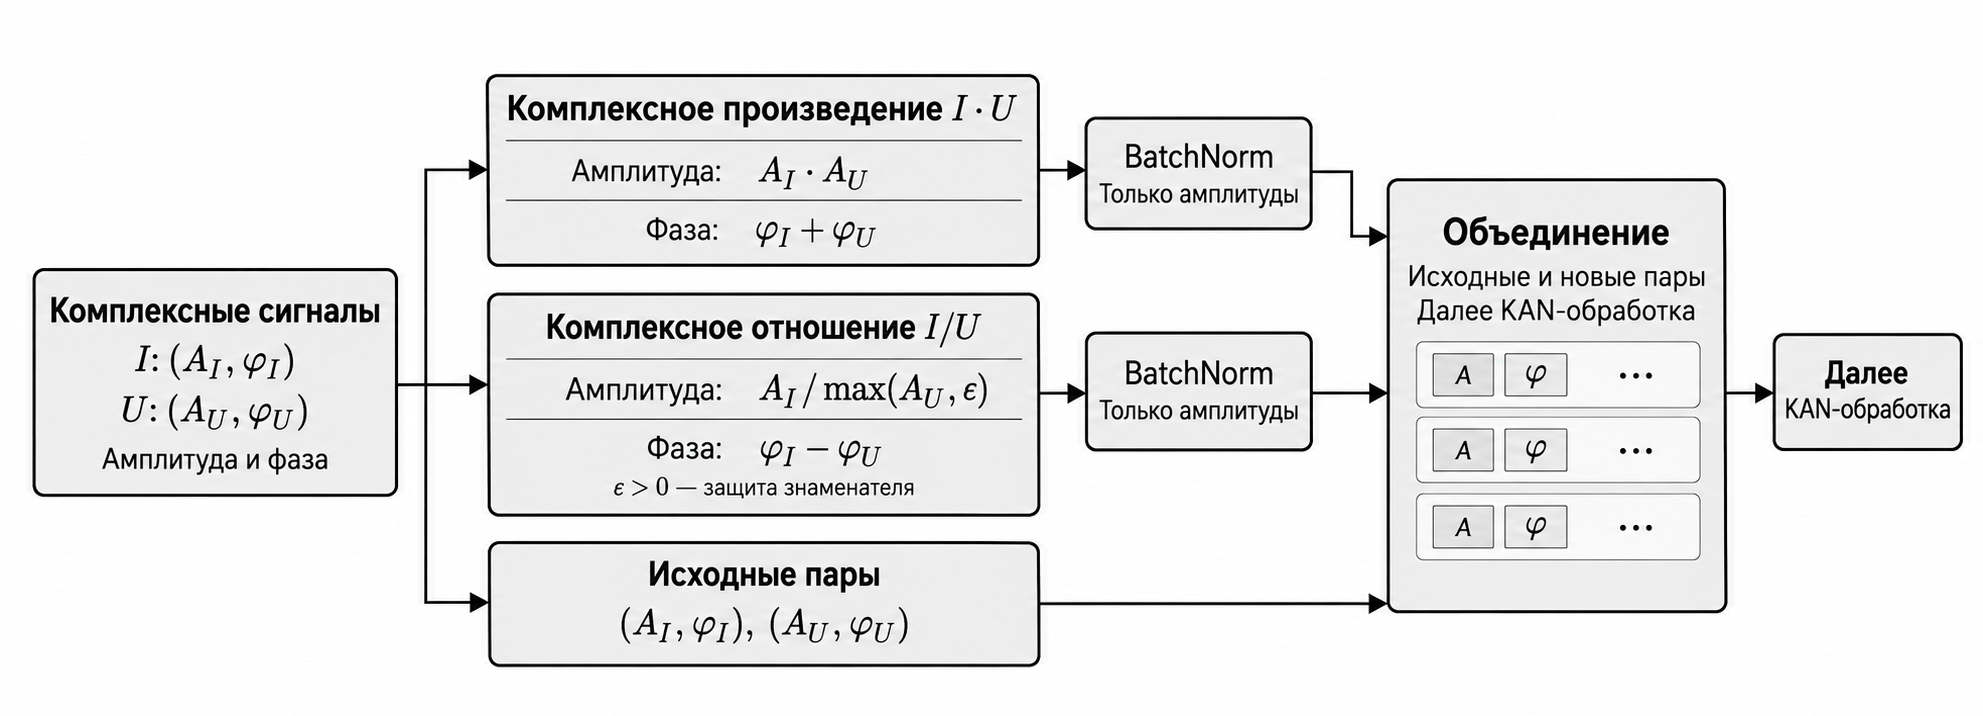
\includegraphics[width=\textwidth]{physkan_complex_ops.png}
    \caption{Комплексные арифметические операции в полярном
    представлении. Показан случай без дополнительного фазового сдвига}
    \label{fig:ch4_complex_flow}
\end{figure}

В комплексном входе амплитуда и фаза каждого сигнала
располагаются рядом. Пары тока и напряжения согласуются
по фазе сети и гармонике. Для трёх токов и трёх напряжений
такое представление содержит 12 вещественных каналов.
Три комплексных произведения и три комплексных отношения
добавляют ещё 12 вещественных каналов. В результате
последующая часть модели получает 24 канала.
Числа здесь поясняют один условный состав входа.
При использовании нескольких гармоник состав расширяется
соответственно выбранному представлению. 

В рассматриваемом комплексном блоке может задаваться
дополнительный фазовый сдвиг, который добавляется
к вычисленной сумме или разности фаз. При нулевом сдвиге
действуют непосредственно формулы~\eqref{eq:ch4_complex_operations}.
Значение этого параметра и порядок входных пар должны
быть согласованы с принятым представлением.

Комплексное произведение следует отличать от комплексной мощности.
При принятом определении векторов тока и напряжения мощность
вычисляется как $\dot{S}=\dot{U}\dot{I}^{*}$,
где звёздочка обозначает комплексное сопряжение.
Поэтому для неё используется разность фаз напряжения и тока.
Обычное произведение в формуле~\eqref{eq:ch4_complex_operations}
содержит сумму фаз. Признаки, полученные таким умножением,
не следует непосредственно именовать активной и реактивной
мощностью. Для получения сопряжённого тока достаточно поменять
знак его фазы перед умножением. Обучаемые преобразования также
могут подобрать нужную зависимость, но при физическом толковании
признака требуется учитывать фактически выполненную операцию.
\iffalse
(Примечание автора: Но в рамках модели это легко решается добавлением «минуса» к требуемому параметру.) **[AA057: закрыто автором; сохранено в истории]**
(Примечание автора: Ок, закрываем)
\fi
\authorreviewnote{AA057}


\iffalse
(Примечание автора: А можно ли комплексные числа писать через точечку над элементами, а не нижнее подчёркивание? А то мне так удобнее. Тут и в других местах.) **[AA073: закрыто автором; сохранено в истории]**
(Примечание автора: Ок, закрываем)
\fi
\authorreviewnote{AA073}

Отношение $\dot{I}/\dot{U}$ соответствует комплексной
проводимости при согласованном выборе измеряемых величин.
Для физического толкования результатов важны порядок каналов,
нормализация и выбранная гармоника. Если электрические сигналы
заменены их обучаемыми комбинациями, операция сохраняет
математический смысл, а электротехническое название признака
уже требует отдельного обоснования.

Например, пусть напряжение имеет амплитуду 10
и фазу ноль, а ток амплитуду 2 и фазу $-30^\circ$.
Обычное произведение имеет амплитуду 20 и фазу $-30^\circ$.
Произведение напряжения на сопряжённый ток имеет ту же
амплитуду, но фазу $+30^\circ$.
Отношение тока к напряжению имеет амплитуду 0,2
и фазу $-30^\circ$. Это арифметический пример,
показывающий значение выбора операции. Он не относится
к зарегистрированному режиму и не задаёт единицы
признаков после нормализации.
\iffalse
(Примечание автора: Но опять же, модель может получить нужные величины сама подогнав раньше и/или после.) **[AA058: закрыто автором; сохранено в истории]**
(Примечание автора: Пусть так, закрываем)
\fi
\authorreviewnote{AA058}


При построении угловой характеристики требуется учитывать
периодичность фазы. Например, углы $179^\circ$ и $-179^\circ$
описывают близкие направления, хотя как числа заметно различаются.
Если обучаемая функция получает сам угол, ей приходится
согласовывать характеристику у двух границ диапазона.
Разделение амплитуд и фаз в rPhysicsKAN помогает выделить
угловое управление в отдельную ветвь, но само по себе
не задаёт периодичность этой функции. В дальнейшем этот вопрос
рассматривается при построении направляющего блока трансформерной
модели в подразделе~\ref{sec:ch4_attention_architecture}.
\iffalse
(Примечание автора: Тут больше проблема для модели как границы задавать и/или кривую, я это помню, но сразу не понятно, надо бы как-то иначе описать проблему. И кстати, а дальше она не решается разве? Вроде бы в следующей модели как раз решается эта проблема) **[AA059: закрыто автором; сохранено в истории]**
(Примечание автора: Ок, закрываем)
\fi
\authorreviewnote{AA059}


Комплексные дополнительные признаки объединяются с исходным
представлением. В рассматриваемой реализации нормализация
результатов физических операций применяется к амплитудам,
а фазы сохраняются отдельными компонентами. Это поддерживает
их различное назначение в последующей обработке.

При обучении комплексного варианта также используется
согласованное отключение компонент пары. Одна случайная маска
применяется и к амплитудной, и к фазовой компоненте
соответствующей позиции. Поэтому отключённая амплитуда
не остаётся представленной вместе с независимо сохранённой
фазой того же признака. Это относится к процедуре обучения
внутреннего представления. При обработке обученной моделью
случайное отключение не применяется.

Нормализованная амплитудная компонента представляет
уже внутренний признак модели. После вычитания среднего
она может иметь отрицательные значения, хотя модуль
исходного комплексного сигнала неотрицателен.
Это ещё одна причина различать физическую величину
на входе арифметики и её последующее обучаемое представление.
Физическое объяснение должно относиться к определённому
этапу вычислений, а не к названию канала на всех слоях.

\subsection{Управление амплитудными признаками по фазе}
\label{sec:ch4_relay_gate}


\iffalse
(Примечание автора: И честно, тут не совсем понятно, а все эти разные подходы являются продолжением или отдельными вариантами? Особенно с вот этой РНМ, кстати да, опиши, что по своей сути, это как раз РНМ, который исследуется в нашей работе, что ОЧЕНЬ важно. А суть вопроса в том, используются ли тут физические сигналы? Произведение / мощности и аналогично с делением? Я уже не помню, и вот подзабыл. Про это, не обязательно тут писать, но где-то надо обще упомянуть. А про РНМ, можно бы и тут) **[AA060: закрыто автором; сохранено в истории]**
(Примечание автора: Да, принимаю так, если что, буду отдельно комментарии оставлять)
\fi
\authorreviewnote{AA060}


Архитектура rPhysicsKAN развивает комплексное представление
за счёт разделения обработки амплитуд и фаз. Внутри сети
формируется обучаемый направляющий орган по принципу РНМ,
в котором угловые соотношения управляют передачей амплитудных
признаков. Такое угловое управление представляет один из способов
построения нейросетевого направляющего органа. Предметная
проверка РНМ рассматривается
в главе~\ref{ch:ml_adaptive_algorithms}.
После формирования дополнительных признаков амплитудная
и фазовая компоненты поступают в отдельные KAN-ветви.
Ещё одна ветвь получает фазовую информацию и формирует
коэффициенты управления амплитудными признаками.

Структура представлена на рисунке~\ref{fig:ch4_relay_flow}.
Сначала выполняются комплексные произведения и отношения,
а их результаты объединяются с исходными парами.
Из общего набора выделяются все амплитудные компоненты
и все фазовые компоненты. Для этих двух наборов
применяется отдельная нормализация. После входной нормализации
амплитудного набора дополнительно используется softplus.
На рисунке этот подготовительный шаг объединён с входом ветви.

\iffalse
(Примечание автора: Урезал картинку, если нужно старое из неё - добавь где-то в текст. Находится в папке "_Устаревшее для памяти") **[AA076: рассмотрено 22.10; ожидает проверки]**
(Примечание автора: Закрывай задачу.)
\fi

\begin{figure}[htbp]
    \centering
    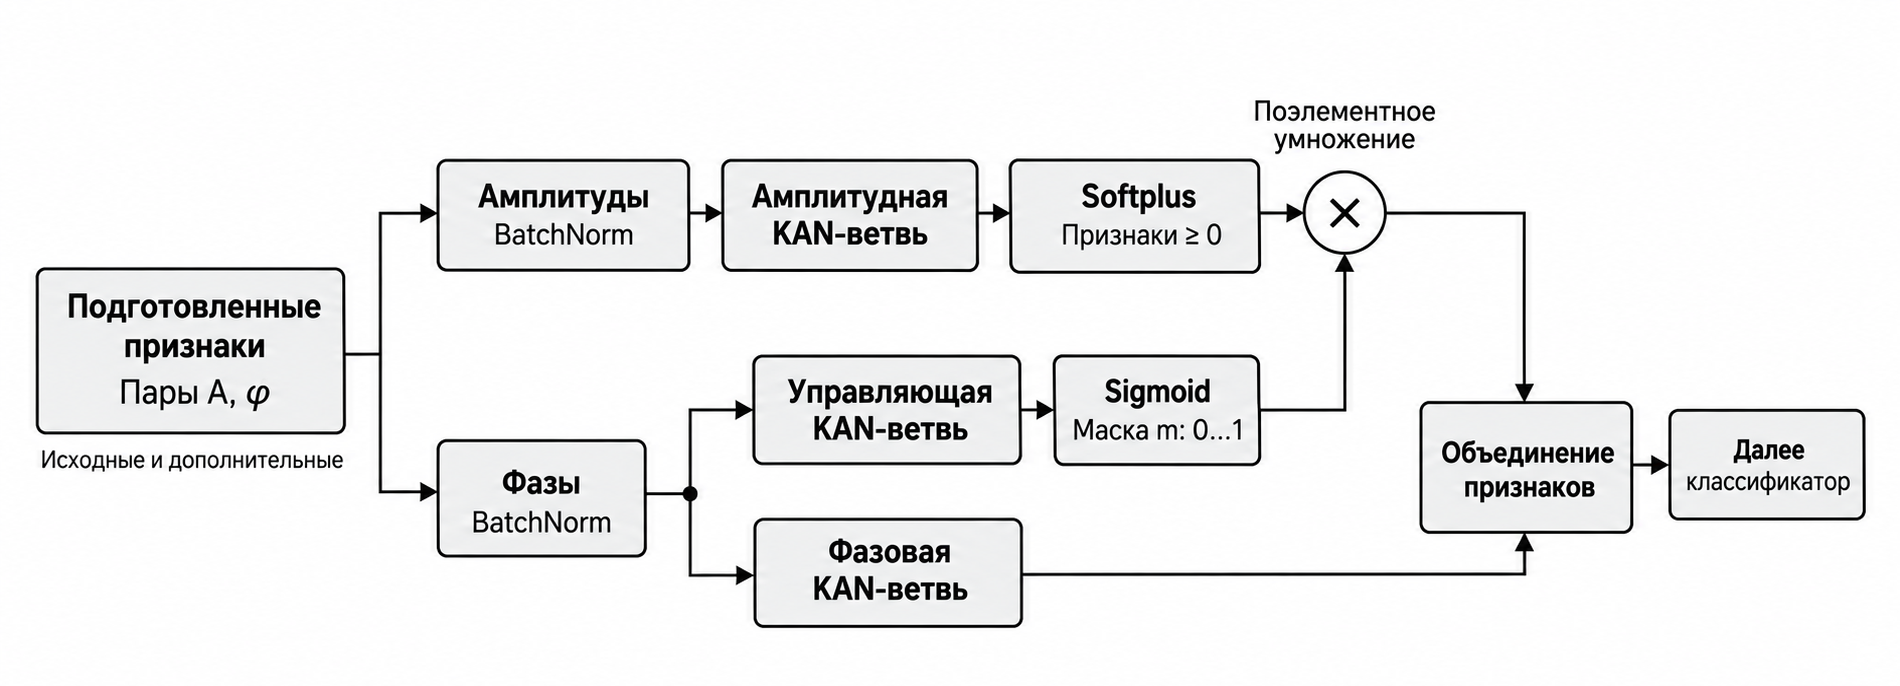
\includegraphics[width=\textwidth]{physkan_relay_gate.png}
    \caption{Раздельные ветви и фазовое управление в rPhysicsKAN.
    Коэффициенты маски умножаются на неотрицательные
    признаки амплитудной ветви. Входная подготовка показана укрупнённо}
    \label{fig:ch4_relay_flow}
\end{figure}

Амплитудная ветвь обрабатывает только амплитудный набор.
Фазовая ветвь формирует признаки для дальнейшего
классификатора. Управляющая ветвь также получает фазовый
набор, но её выход используется для изменения передачи
амплитудной информации. Фазовая и управляющая ветви
имеют разное назначение и собственные обучаемые параметры.
Подача одинакового исходного набора не делает
их преобразования одинаковыми.

Амплитудная и управляющая ветви формируют одинаковое число признаков,
чтобы каждый коэффициент маски мог изменять соответствующий
амплитудный отклик. Состав слоёв и уменьшение длины окна
выбираются при задании конфигурации модели.
\iffalse
(Примечание автора: Разве надо тут так закапываться в подробности? Возможно надо как-то аккуратнее описать) **[AA061: закрыто автором; сохранено в истории]**
(Примечание автора: Ок, это замечание закрываем, дальше по ходу писать буду в случае чего)
\fi
\authorreviewnote{AA061}


Пусть $\boldsymbol{a}$ и $\boldsymbol{\varphi}$ обозначают
векторы входных амплитуд и фаз после подготовки признаков.
Обучаемые преобразования амплитудной и управляющей ветвей
обозначим $F_a$ и $F_g$. В рассматриваемой реализации
управляемая амплитудная ветвь имеет вид
\begin{equation}
    \widetilde{\boldsymbol{a}} =
    \operatorname{softplus}\bigl(F_a(\boldsymbol{a})\bigr)
    \odot \sigma\bigl(F_g(\boldsymbol{\varphi})\bigr),
    \label{eq:ch4_relay_gate}
\end{equation}
где $\odot$ обозначает поэлементное умножение,
$\sigma(x)=1/(1+e^{-x})$,
а $\operatorname{softplus}(x)=\ln(1+e^x)$.
Сигмоидальная функция ограничивает коэффициенты управления
диапазоном от нуля до единицы. Преобразование softplus
обеспечивает неотрицательное значение управляемых признаков.
Полученный результат объединяется с выходом фазовой ветви
и поступает в последующую часть классификатора.

В отличие от жёсткой блокировки маска действует
непрерывно. При выходной оценке управляющей ветви $g=0$
сигмоидальный коэффициент равен 0,5. Для $g=2$
он составляет приблизительно 0,88, а для $g=-2$
приблизительно 0,12. Эти значения иллюстрируют формулу,
а не измеренную характеристику обученного органа.
По мере изменения фазовых признаков модель может
плавно ослаблять или пропускать амплитудную составляющую.

Softplus применяется перед умножением на маску.
Он переводит выход амплитудной ветви в неотрицательное
представление, сохраняя возможность плавного изменения.
Так величина коэффициента маски определяет степень
передачи признака. Без этого преобразования отрицательное
значение скрытой амплитудной компоненты могло бы иметь
другой смысл при последующем умножении.

После управления амплитудные признаки вновь объединяются
с выходами фазовой ветви. В варианте с временными картами
выполняются итоговое усреднение и KAN-классификация.
В варианте с развёрнутым коротким представлением
используется соответствующая полносвязная KAN-обработка.
В обоих случаях выходом остаются оценки выбранных событий.
Маска является внутренним механизмом модели,
а не непосредственной командой выключателю.

Такая структура задаёт зависимость передачи амплитудной
информации от фазовых соотношений. По своему назначению
она близка к использованию угла между электрическими
величинами в направленном измерительном органе.
При этом обучаемый коэффициент управления не равен
заранее заданной функции $\cos\varphi$ и не обеспечивает
сам по себе тождественность классическому РНМ.
Его характеристика определяется обучением и должна
исследоваться на соответствующих режимах.

Для БАВР такая архитектурная идея интересна возможностью
совместно учитывать амплитудные признаки и направление,
связанное с фазовыми соотношениями. Классификация событий
в осциллограмме и решение о разрешении либо блокировке
переключения имеют разные целевые выходы. Поэтому перенос
архитектуры на задачу РНМ предполагает собственную разметку,
условия применимости и проверку поведения органа во времени.


\iffalse
(Примечание автора: Да, ещё раз повторю, что тут мы как бы создали отдельный орган РНМ внутри нашей нейросетки. Хотя... ты и так пишешь об этом, извиняюсь. Возможно надо куда-то и в начало этого подраздела перенести тоже краткий комментарий об этом.) **[AA062: закрыто автором; сохранено в истории]**
(Примечание автора: Считаем закрытой, убираем)
\fi
\authorreviewnote{AA062}


\subsection{Анализ последовательностей и Physical KAN-Transformer}
\label{sec:ch4_attention_architecture}

\iffalse
(Примечание автора: Ок, хорошо, а для модели «Physical KAN-Transformer» пока что нет совсем картинок, наверное надо бы какую-то поясняющую что такое трансформерная архитектура. Да и надо бы подробнее про эту модель из статьи той описать, а то уж очень кратко, а ведь там много чего говорится, и ранее ссылаемся, что подробнее разберём в главе 3.9, а там почти ничего и нет. И картинок – хорошо бы добавить точно поясняющих. Ну реально, сейчас глянул, и да, там ведь прям очень много сравнений… Да, там сперва описывается обычная трансформерная модель, а потом наша, но всё же, людям надо бы сперва пояснить ту особенность, причём повторюсь, не обязательно сразу пихать те картинки – можно бы сперва подробно описать, что нужно нарисовать, нарисуем, и с нужным именем сохраним в нужную папку. И да, пока можешь какую-то заглушку вставить, не так важно, я создам потом картинку лучше.) **[AA064: закрыто автором; сохранено в истории]**
(Примечание автора: Считаем устаревшей и закрываем, буду по ходу текста писать в случае чего.)
\fi
\authorreviewnote{AA064}

Скользящее окно ограничивает доступную модели предысторию.
В рассмотренных выше классификаторах из окна формируется одна
совокупность оценок. При перемещении окна положение повреждения
внутри него изменяется, а вместе с ним может изменяться выход.
Для кратковременных дуговых пробоев и затухающих процессов важно
также соотношение нескольких последовательных участков записи.
Одинаковый провал напряжения может сопровождать разные процессы,
различающиеся предшествующим изменением токов и дальнейшим
восстановлением режима.

В работе об архитектурной эволюции интеллектуальных
защит\footnote{Евдаков А.Е., Яблоков А.А., Филатова Г.А.
Архитектурная эволюция интеллектуальных защит. Интеграция сетей
Колмогорова--Арнольда и механизма внимания.} переход к анализу
последовательностей реализован с помощью трансформерной модели.
Она сопоставляет представления отдельных временных участков
и использует найденные связи при формировании выхода для каждой
зоны. В рассматриваемой постановке буфер содержит десять периодов
промышленной частоты, а зона соответствует половине периода.
Такой буфер содержит двадцать зон. Это параметры постановки
конкретного исследования, а не неизменные размеры архитектуры.

\paragraph{Последовательность признаков и механизм внимания.}
Для каждого положения в буфере формируется вектор признаков,
который далее будем называть токеном. В задаче анализа осциллограмм
он описывает соответствующий участок токов и напряжений.
Последовательность токенов сохраняет порядок развития процесса.
Представление положения позволяет различать одинаковые признаки,
возникшие в начале и в конце доступной предыстории.

Механизм внимания определяет, какие участки последовательности
существенны для обновления текущего представления. Из каждого
токена тремя обучаемыми преобразованиями получаются запрос,
ключ и значение. Запрос задаёт, какую информацию ищет текущее
положение. Ключ используется для сопоставления с ним других
положений. Значение содержит признаки, которые передаются
после такого сопоставления. Поэтому вес внимания и передаваемая
информация выполняют разные функции.

Для запроса $\boldsymbol{q}_t$ текущего положения и ключей
$\boldsymbol{k}_s$ доступных положений веса имеют вид
\begin{equation}
    \alpha_{ts}=\frac{\exp\!\left(
    \boldsymbol{q}_t\boldsymbol{k}_s^{\mathsf T}/\sqrt{d}\right)}
    {\displaystyle\sum_{u\in\mathcal{A}_t}\exp\!\left(
    \boldsymbol{q}_t\boldsymbol{k}_u^{\mathsf T}/\sqrt{d}\right)},
    \qquad
    \boldsymbol{z}_t=\sum_{s\in\mathcal{A}_t}
    \alpha_{ts}\boldsymbol{v}_s.
    \label{eq:ch4_attention_weights}
\end{equation}
Здесь $d$ является размерностью запроса и ключа,
$\boldsymbol{v}_s$ вектором значений, а $\mathcal{A}_t$
множеством разрешённых положений. Нормировка Softmax делает
сумму весов равной единице. На выходе получается взвешенная
сумма значений, которая объединяет информацию разных участков.
Таким образом, модель может связать текущий провал напряжения
с предшествующим броском тока. Сам по себе такой вес показывает
обращение к признакам, а физическое объяснение связи проверяется
по соответствующему режиму.

\begin{figure}[htbp]
    \centering
    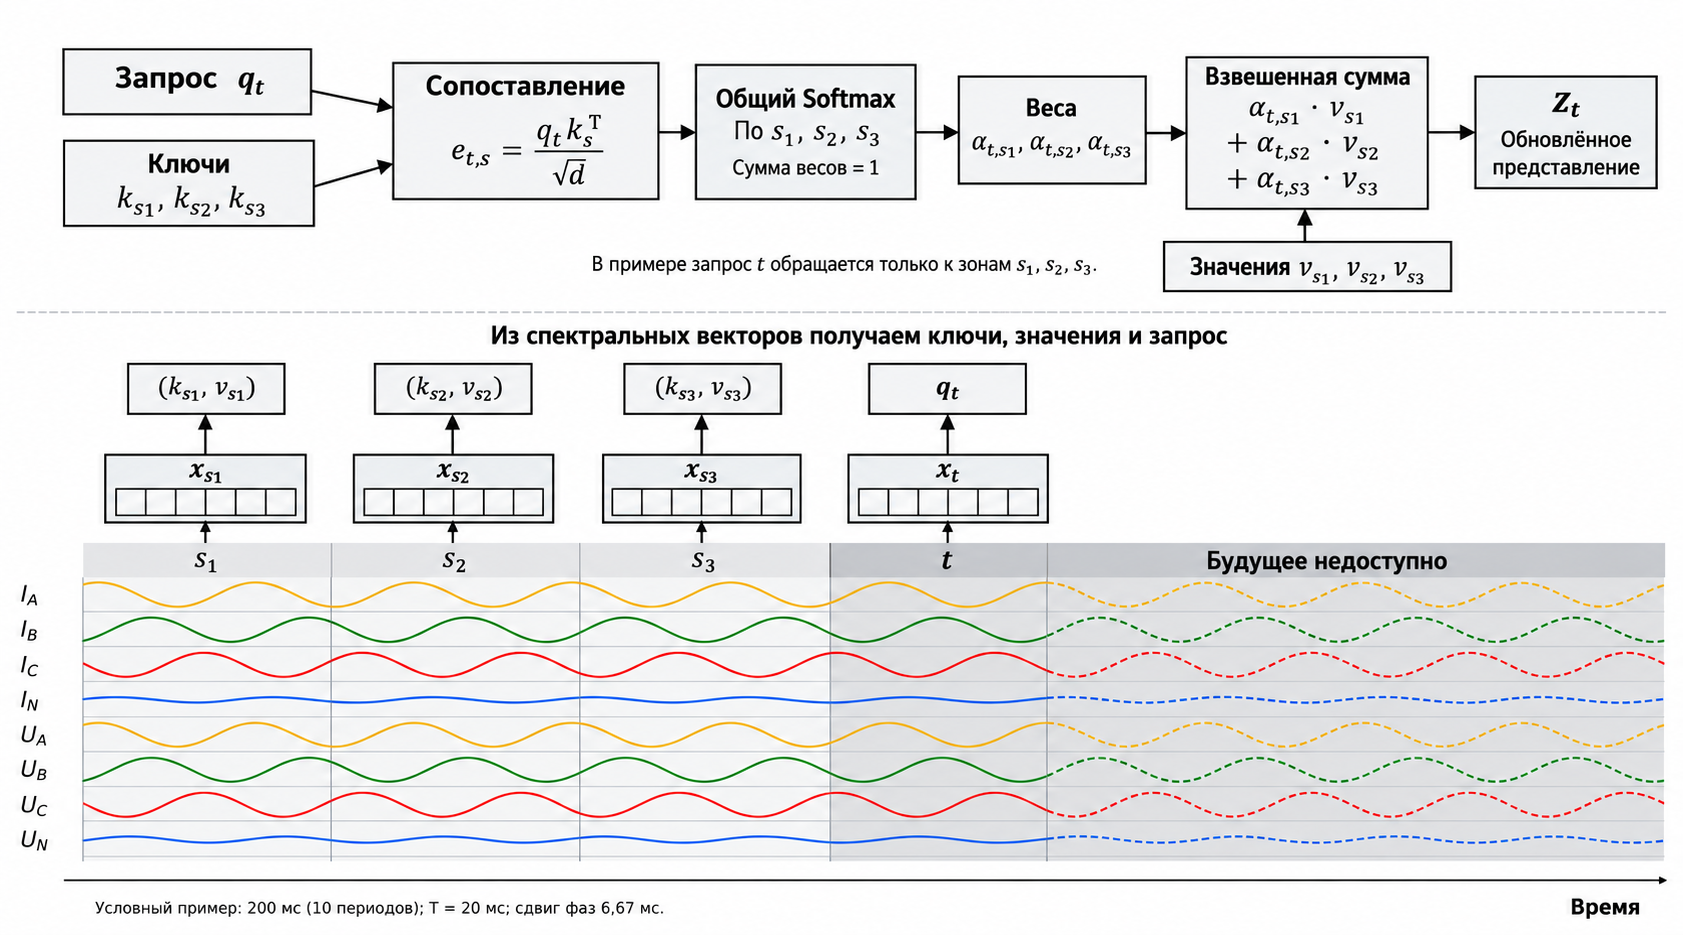
\includegraphics[width=\textwidth]{transformer_attention.png}
    \caption{Принцип внимания при обработке последовательности признаков осциллограммы. Условная схема доступа к предыстории}
    \label{fig:ch4_transformer_attention}
\end{figure}

При многоголовом внимании несколько таких преобразований
работают параллельно со своими параметрами. Их результаты
объединяются в общее представление. Это даёт несколько способов
сопоставления временных участков, но заранее не закрепляет
за отдельной головой определённое физическое явление.
На рисунке показан вариант обращения только к предыдущим зонам.
Причинное самовнимание используется, в частности, и в декодерных
трансформерах. Однако наличие такой маски само по себе
не определяет полный состав архитектуры. В рассматриваемой
модели основную обработку выполняет кодирующая часть трансформера.
\iffalse
(Примечание автора: Ведь такая архитектура называется декодер? я же прав, можно бы пару слов коротко, прям очень коротко. Можно сделать чуть иначе, и все на всё чтобы смотрели, но мы в будущем будем решать релейные защиты, поэтому пока что так, хотя для разметки, быть может, лучше бы чуть иначе. Можно где-то в другом месте эту тематику внимания затронуть, а про релейность - вообще общий момент на самом деле.) **[AA077: рассмотрено 22.10; ожидает проверки]**
(Примечание автора: Закрываем вопрос, хорошо.)
\fi
\authorreviewnote{AA077}
При обработке полученного буфера в рассматриваемой архитектуре
связи разрешены между всеми его непотерянными позициями.
Поэтому внутренняя зона может использовать более позднюю зону
того же буфера. Ограничение доступной информации границей
наблюдаемого окна и запрет будущих позиций относительно каждой
внутренней зоны являются разными условиями. Одна иллюстрация
обращения к предыстории не устанавливает потоковый характер
всех опытов.

\paragraph{Базовая трансформерная архитектура.}
Во входном блоке базовой модели линейное преобразование
спектрального вектора сопровождается GELU, нормализацией
и Dropout. Затем добавляется представление положения зоны
и выполняется последовательность блоков внимания. В каждом блоке обмен информацией между
временными участками сочетается с полносвязным преобразованием
признаков каждого участка. Остаточные связи передают вход
блока к его выходу, а нормализация согласует масштабы внутренних
откликов. Эта организация показана на
рисунке~\ref{fig:ch4_transformer_baseline}.

\begin{figure}[htbp]
    \centering
    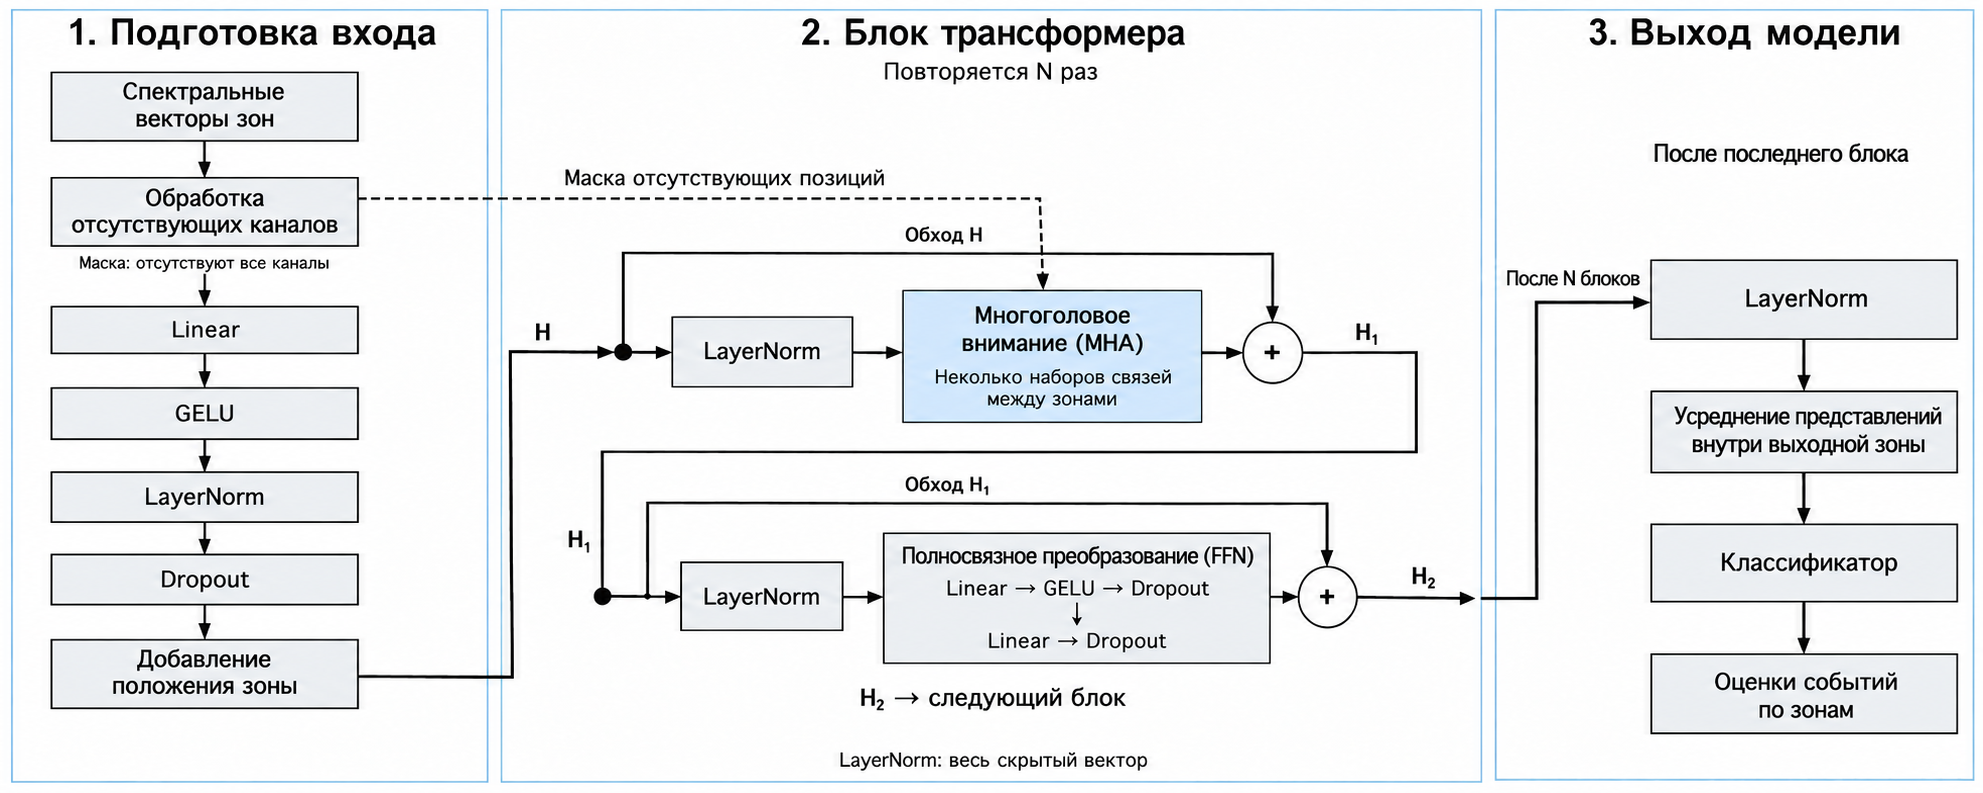
\includegraphics[width=\textwidth]{transformer_baseline_detail.png}
    \caption{Последовательность обработки в базовой трансформерной модели}
    \label{fig:ch4_transformer_baseline}
\end{figure}

\iffalse
(Примечание автора: Урезал картинку, если нужно старое из неё - добавь где-то в текст. Находится в папке "_Устаревшее для памяти") **[AA076: рассмотрено 22.10; ожидает проверки]**
(Примечание автора: Закрывай задачу.)
\fi

В отличие от свёртки с локальным ядром, внимание непосредственно
сопоставляет разные положения доступного буфера. За это
приходится платить вычислением попарных связей между токенами.
Увеличение числа зон меняет и объём таких вычислений.
Следовательно, длина предыстории и шаг её представления влияют
на вычислительную сложность наряду с числом параметров сети.

Обычная линейная проекция и полносвязные слои не выделяют
амплитуды и фазы как разные по смыслу величины. Они могут
обучаться нужным зависимостям, однако в их структуре отдельно
не заданы комплексные произведения, отношения и направляющее
действие угла. Для включения этих операций разработана
Physical KAN-Transformer.

\paragraph{Полярный вход и дополнительные признаки.}
Вход Physical KAN-Transformer содержит пары амплитуды $A$
и фазы $\varphi$ спектральных составляющих токов и напряжений.
Помимо первых девяти гармоник используются низкочастотные
составляющие на интервалах два, четыре, шесть и десять периодов
и симметричные составляющие основной гармоники. Фазы имеют
общий отсчёт относительно напряжения фазы A. Один временной
вектор поэтому описывает несколько измеряемых величин,
а не одну точку отдельного сигнала.

Перед обработкой отмечаются отсутствующие каналы. Пропуск
заменяется безопасным числовым значением с обучаемым маркером,
чтобы отличать отсутствие измерения от измеренного нуля.
Из внимания исключаются позиции, в которых отсутствуют все каналы.
Далее входной каскад PhysicalStem формирует скрытое представление,
к нему добавляется код положения, после чего работают повторяемые
блоки внимания и физического преобразования признаков.
Для понимания входного каскада сначала рассмотрим две его операции.

\paragraph{Произведения и отношения комплексных величин.}
Пара $(A,\varphi)$ задаёт комплексный вектор. Комплексный блок
сначала формирует несколько обучаемых комбинаций таких векторов.
Одни и те же вещественные веса применяются к действительным
и мнимым частям. Это сложение комплексных векторов с весами,
при котором модуль и угол результата зависят от всех слагаемых.
Промежуточные результаты разделяются на четыре группы.
Векторы первой и второй групп попарно перемножаются,
а векторы третьей группы делятся на соответствующие векторы
четвёртой. Произведение и отношение вычисляются параллельно,
как показано на рисунке~\ref{fig:ch4_transformer_interactions}.

\iffalse
(Примечание автора: Во первых, надо бы как-то пояснить сразу, что мы не удаляем токи и напряжения, а добавляем ещё и вот такие признаки. А то кажется, что мы ТОЛЬКО произведение и деление дальше используем.
Во вторых, надо будет здесь оставить другое примечание – о том, чтобы пояснения из картинки, какие важные, если их нет – перенести в текст, а оставить только схему, и совсем важные комментарии. Я про текст начиная от «Всего n комплексных результатов: …» на картинке. Он явно не нужен на картинке и начал появляться с 4.13 картинки вроде как. Если можешь – усеки сама картинки, ток оставь старые, чтоб не потерять их, а если будет норм – то потом оставим только новые. Пожалуй, скину картинку в чат с пояснением даже.) **[AA074: закрыто автором; сохранено в истории]**
(Примечание автора: Ок, сейчас закрываем этот момент и убираем замечание.)
\fi
\authorreviewnote{AA074}

\iffalse
(Примечание автора: Урезал картинку, если нужно старое из неё - добавь где-то в текст. Находится в папке "_Устаревшее для памяти") **[AA076: рассмотрено 22.10; ожидает проверки]**
(Примечание автора: Закрывай задачу.)
\fi

\begin{figure}[htbp]
    \centering
    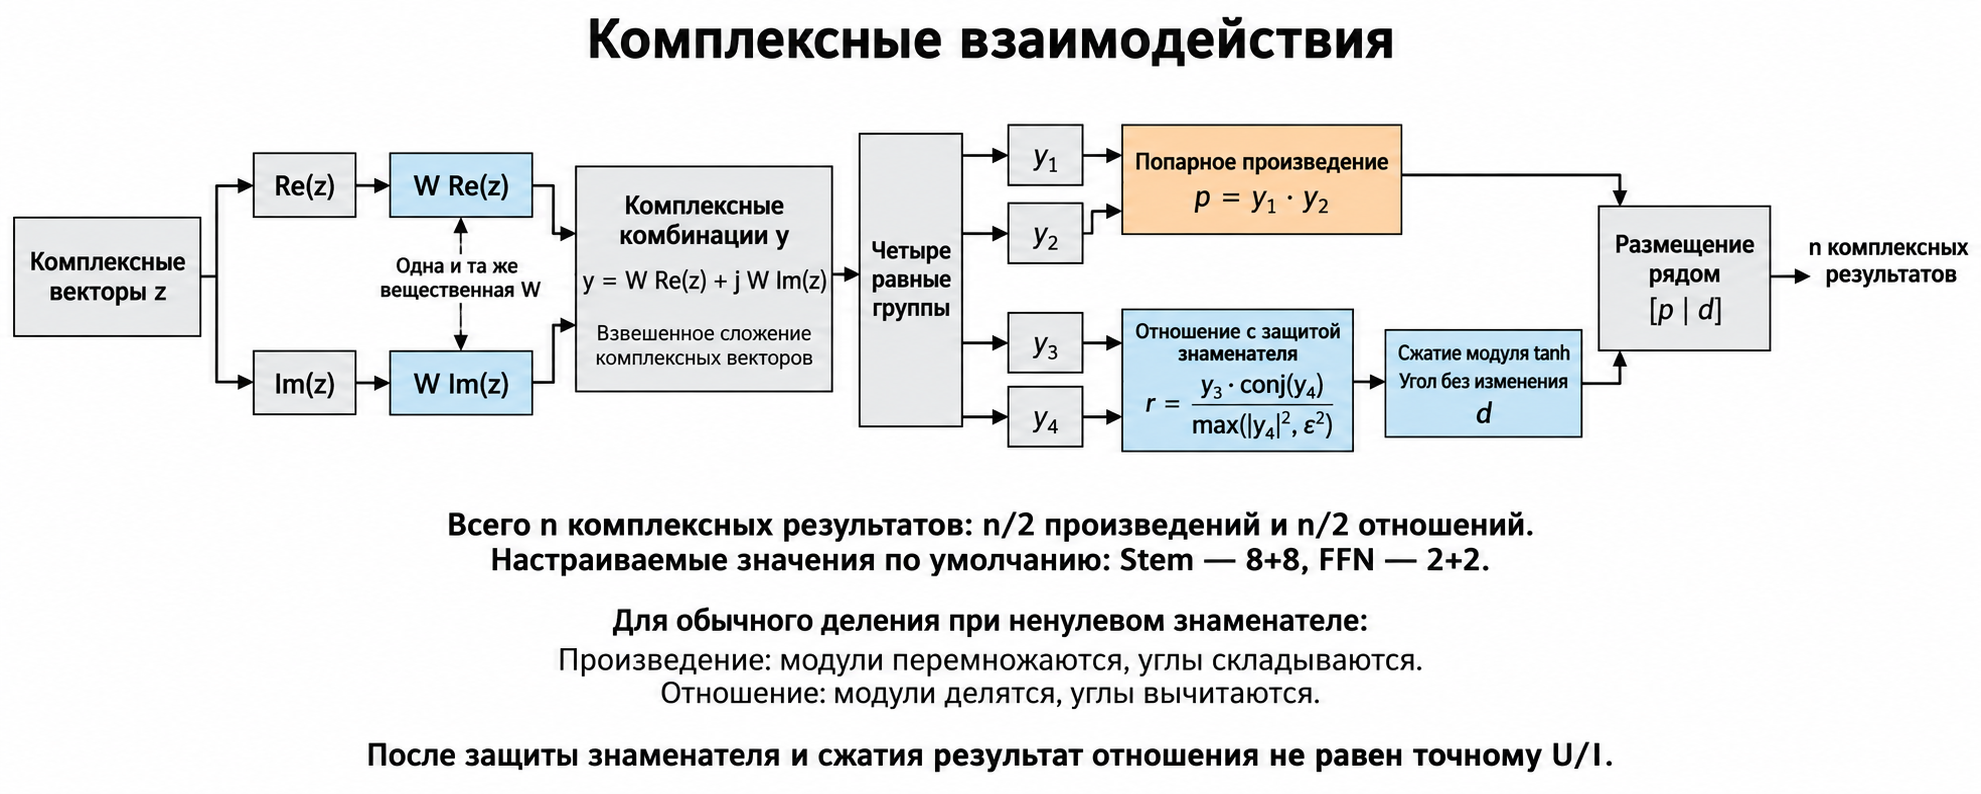
\includegraphics[width=\textwidth]{transformer_interactions_detail.png}
    \caption{Параллельные произведения и отношения в комплексном блоке}
    \label{fig:ch4_transformer_interactions}
\end{figure}

У произведения перемножаются модули и складываются углы.
У обычного отношения модули делятся, а углы вычитаются.
В программном блоке малый знаменатель защищён нижним порогом
его квадрата модуля. После деления модуль дополнительно сжимается
функцией $\tanh$, сохраняющей угол результата. Поэтому выход
этой ветви является ограниченным производным признаком,
а не непосредственно значением сопротивления или проводимости.
Произведения и обработанные отношения размещаются рядом
в выходном наборе. Исходные векторы в него автоматически
не добавляются. Этот рисунок раскрывает только блок дополнительных
признаков, а не весь вход модели. В PhysicalStem исходные амплитуды
и фазы одновременно поступают в другие пути обработки.
Амплитудная KAN-ветвь получает измерительные признаки после
углового управления, а угловая проекция получает также исходные
сдвинутые фазы. Поэтому дальнейшая обработка использует
не только результаты произведений и отношений. Однако отдельная
неизменная копия исходных амплитуд перед проекцией здесь
не присоединяется.

\paragraph{Угол как коэффициент передачи.}
В направляющем блоке угол управляет тем, какая доля амплитудного
признака передаётся дальше. Для каждого канала обучаются центр
угловой зоны $\mu$, её полуширина $\beta$, плавность перехода $s$
и нижний уровень передачи $r$. Коэффициент имеет вид
\begin{equation}
 g(\varphi)=r+(1-r)\,\sigma\!\left[
 s\bigl(\cos(\varphi-\mu)-\cos\beta\bigr)\right],
 \label{eq:ch4_directional_coefficient}
\end{equation}
где $\sigma$ является сигмоидальной функцией. Внутри выбранной
угловой области передача выше, вне её ниже. Переход плавный,
а значение $r$ не обязано быть нулём.

На рисунке~\ref{fig:ch4_directional_geometry} одна и та же операция
показана на комплексной плоскости и как угловая характеристика.
Для условного примера приняты центр зоны $30^\circ$,
полуширина $60^\circ$, нижний уровень 0,2 и параметр плавности 8.
Эти значения поясняют действие формулы, а не представляют
результат обучения модели.
Умножение на положительный коэффициент уменьшает длину вектора,
сохраняя его направление. Например, при коэффициенте 0,6
передаётся 60\% входной амплитуды. Обучаемый поворот входной
фазы и такое ослабление имеют разное назначение. Поворот меняет
угол, а коэффициент передачи меняет модуль.

\begin{figure}[htbp]
    \centering
    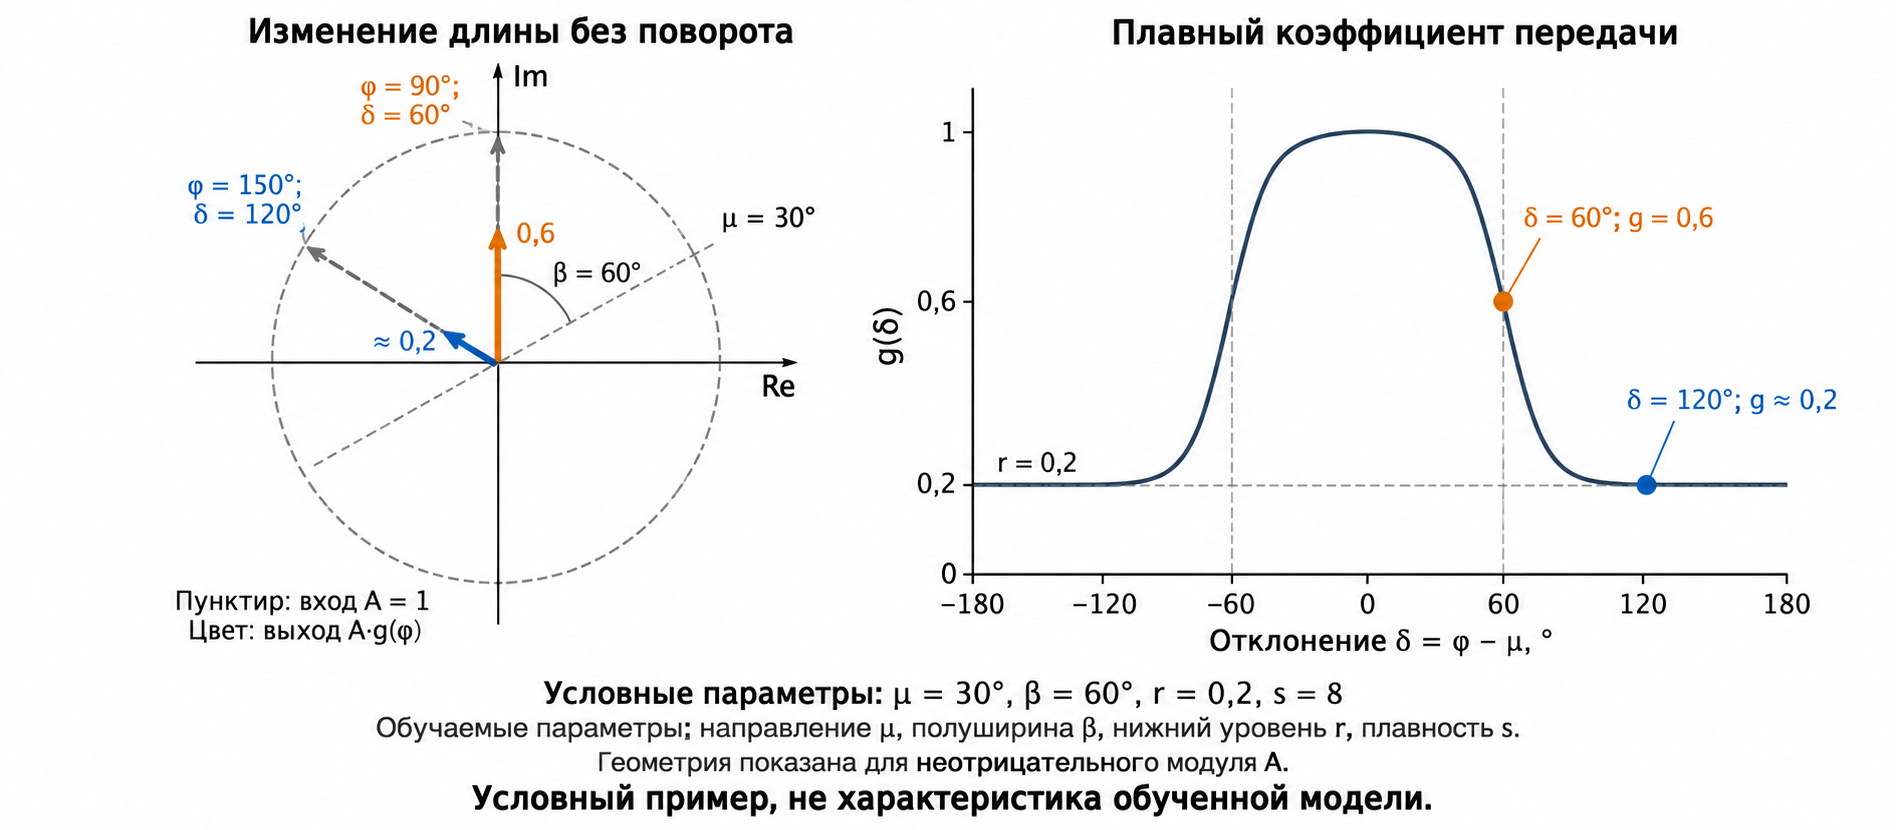
\includegraphics[width=\textwidth]{transformer_gate_geometry.png}
    \caption{Действие плавного углового управления. Параметры и векторы условные}
    \label{fig:ch4_directional_geometry}
\end{figure}

Это развитие идеи направляющего органа, но не готовая команда
РНМ. Здесь регулируется отдельный путь признаков внутри сети.
Рассмотренная ранее rPhysicsKAN получает маску из KAN-ветви
по фазовым признакам. В трансформерном варианте угловая
характеристика задана периодической функцией
\eqref{eq:ch4_directional_coefficient}. Эти два способа управления
нельзя считать одной и той же формулой.

\paragraph{Движение данных во входном PhysicalStem.}
Каскад получает амплитуды и углы каждой зоны. К углам добавляется
обучаемый сдвиг, так что $\varphi'=\varphi+b$. Дальше сдвинутые
углы используются сразу в трёх местах, показанных на
рисунке~\ref{fig:ch4_transformer_physical}.

В амплитудном пути коэффициенты $g(\varphi')$ умножаются
на исходные амплитуды. Полученные значения обрабатывает FastKAN.
Параллельный комплексный путь получает исходные амплитуды
до этого умножения и те же углы $\varphi'$. Он выполняет
произведения и отношения по уже рассмотренной схеме
и возвращает их модули и аргументы. Наконец, сами углы
$\varphi'$ передаются к угловому выходу каскада отдельным путём.
Это ответвление сохраняет сведения об исходных фазах наряду
с фазами новых комплексных признаков.

\iffalse
(Примечание автора: Урезал картинку, если нужно старое из неё - добавь где-то в текст. Находится в папке "_Устаревшее для памяти") **[AA076: рассмотрено 22.10; ожидает проверки]**
(Примечание автора: Закрывай задачу.)
\fi

\begin{figure}[htbp]
    \centering
    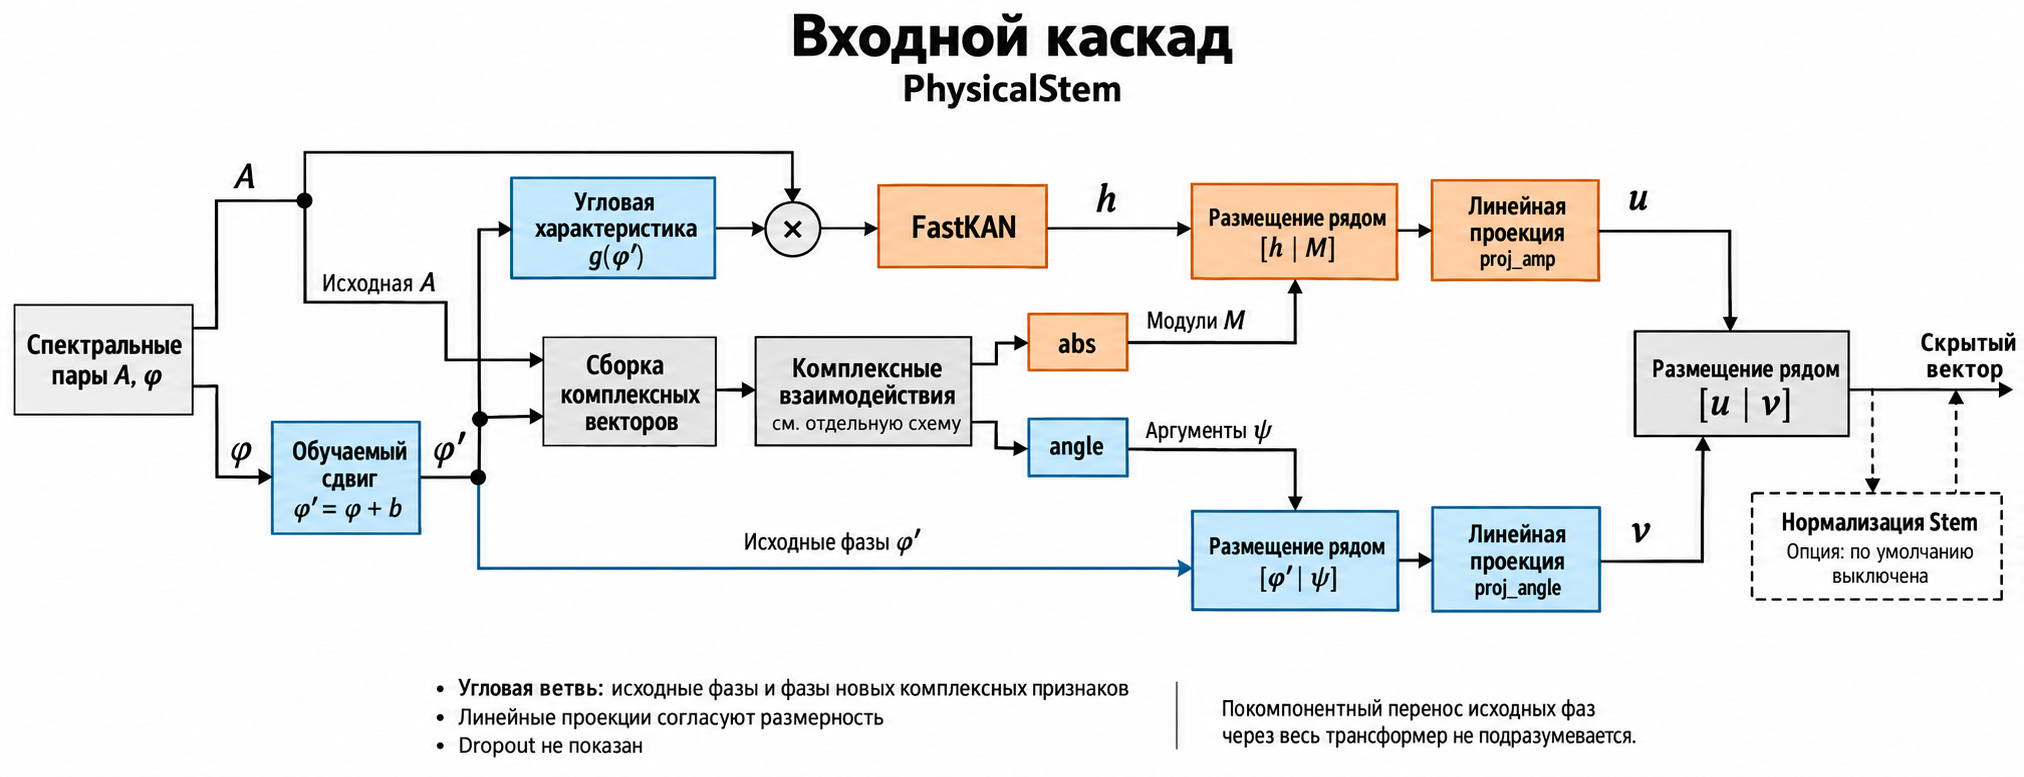
\includegraphics[width=\textwidth]{transformer_stem_detail.png}
    \caption{Входной PhysicalStem. Именованные выходы ветвей используются
    при раздельной сборке двух частей скрытого вектора}
    \label{fig:ch4_transformer_physical}
\end{figure}

При сборке амплитудной части рядом размещаются отклики FastKAN
и модули комплексных результатов. При сборке угловой части
рядом размещаются $\varphi'$ и аргументы комплексных результатов.
Для каждой части выполняется своя линейная проекция к нужному
числу скрытых признаков. Две полученные части $u$ и $v$ вновь
размещаются рядом. Такое объединение не складывает модуль
с углом и не означает прохождения углов через амплитудный FastKAN.
Нормализация выхода самого PhysicalStem опциональна
и в базовом варианте отключена.

Входной каскад одновременно добавляет производные признаки
и согласует размерность данных с повторяемыми блоками.
Прямой угловой путь сохраняет исходные фазовые сведения
на этапе сборки, но последующая проекция уже меняет их состав.
Поэтому скрытая координата $v$ не обязана оставаться фазой
конкретного тока или напряжения.

\paragraph{Многоголовое внимание.}
Внимание связывает временные зоны между собой.
Сокращение MHA образовано от Multi-Head Attention и означает
многоголовое внимание. Каждая голова формирует свои запросы,
ключи и значения и может выделять разные связи между зонами.
Их результаты собираются в общее представление.

В полярном варианте части $u$ и $v$ имеют отдельные проекции
запросов, ключей и значений. Для каждой пары зон складываются
две оценки сходства, полученные из амплитудной и угловой частей.
Сумма масштабируется и нормируется Softmax. Одинаковые веса
затем применяются к значениям обеих ветвей. После сборки голов
выполняются две выходные проекции, показанные на
рисунке~\ref{fig:ch4_polar_attention}.

\iffalse
(Примечание автора: Урезал картинку, если нужно старое из неё - добавь где-то в текст. Находится в папке "_Устаревшее для памяти") **[AA076: рассмотрено 22.10; ожидает проверки]**
(Примечание автора: Закрывай задачу.)
\fi

\begin{figure}[htbp]
    \centering
    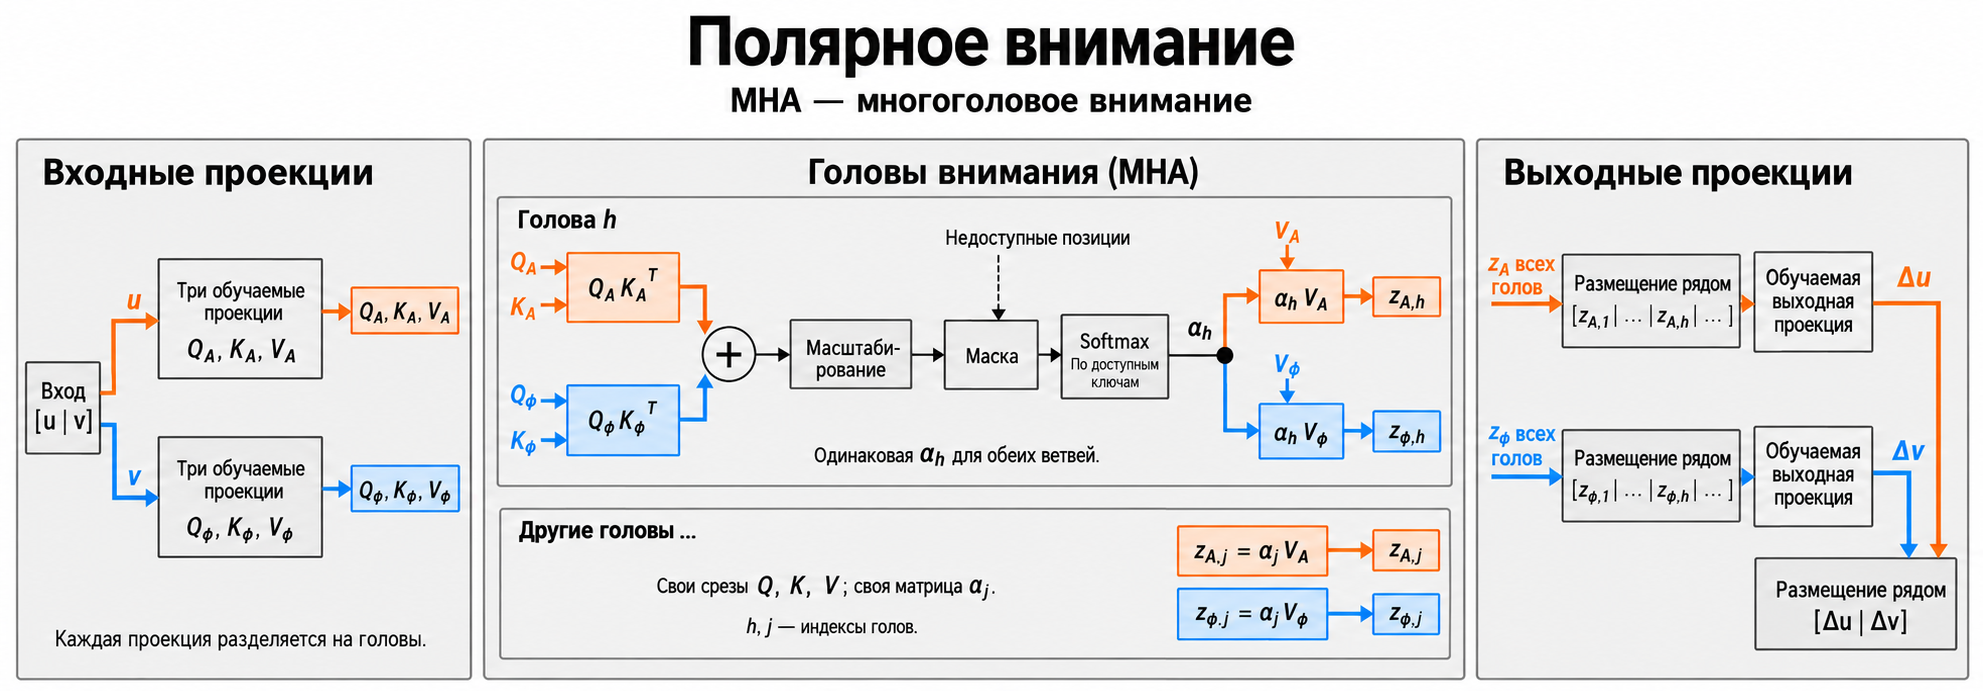
\includegraphics[width=\textwidth]{transformer_attention_detail.png}
    \caption{Полярное многоголовое внимание с общими весами двух ветвей}
    \label{fig:ch4_polar_attention}
\end{figure}

В этом сложении участвуют оценки сходства, а не физические
модули и углы. На внешней остаточной связи к прежним $u$ и $v$
прибавляются соответствующие выходные части внимания.
Направляющего коэффициента $g$ внутри внимания нет.
Он применяется во входном каскаде и следующем физическом блоке.

\paragraph{Физический блок после внимания.}
Полносвязный блок FFN, от Feed-Forward Network, преобразует
признаки каждой зоны после обмена информацией с другими зонами.
В физическом варианте его устройство показано на
рисунке~\ref{fig:ch4_physical_ffn}.
При обучении после каждого FastKAN применяется Dropout.
При оценке обученной модели эта случайная обработка выключена.
Амплитудная часть $u$ проходит два FastKAN-слоя,
а результат умножается на $g(v)$. Здесь направляющий коэффициент
вычисляется из входной угловой части FFN без предварительного
добавления его собственного сдвига $b$.

Параллельный комплексный путь получает $u$ и $v$, выполняет
произведения и отношения и использует модули результатов.
После линейной проекции этот вклад умножается на отдельный
обучаемый скаляр и прибавляется к управляемой KAN-ветви.
Угловой выход FFN содержит только обучаемое приращение $b$.
Внешняя остаточная связь добавляет его к прежней угловой части,
а амплитудный вклад к прежней амплитудной части.

\iffalse
(Примечание автора: Урезал картинку, если нужно старое из неё - добавь где-то в текст. Находится в папке "_Устаревшее для памяти") **[AA076: рассмотрено 22.10; ожидает проверки]**
(Примечание автора: Закрывай задачу.)
\fi

\begin{figure}[htbp]
    \centering
    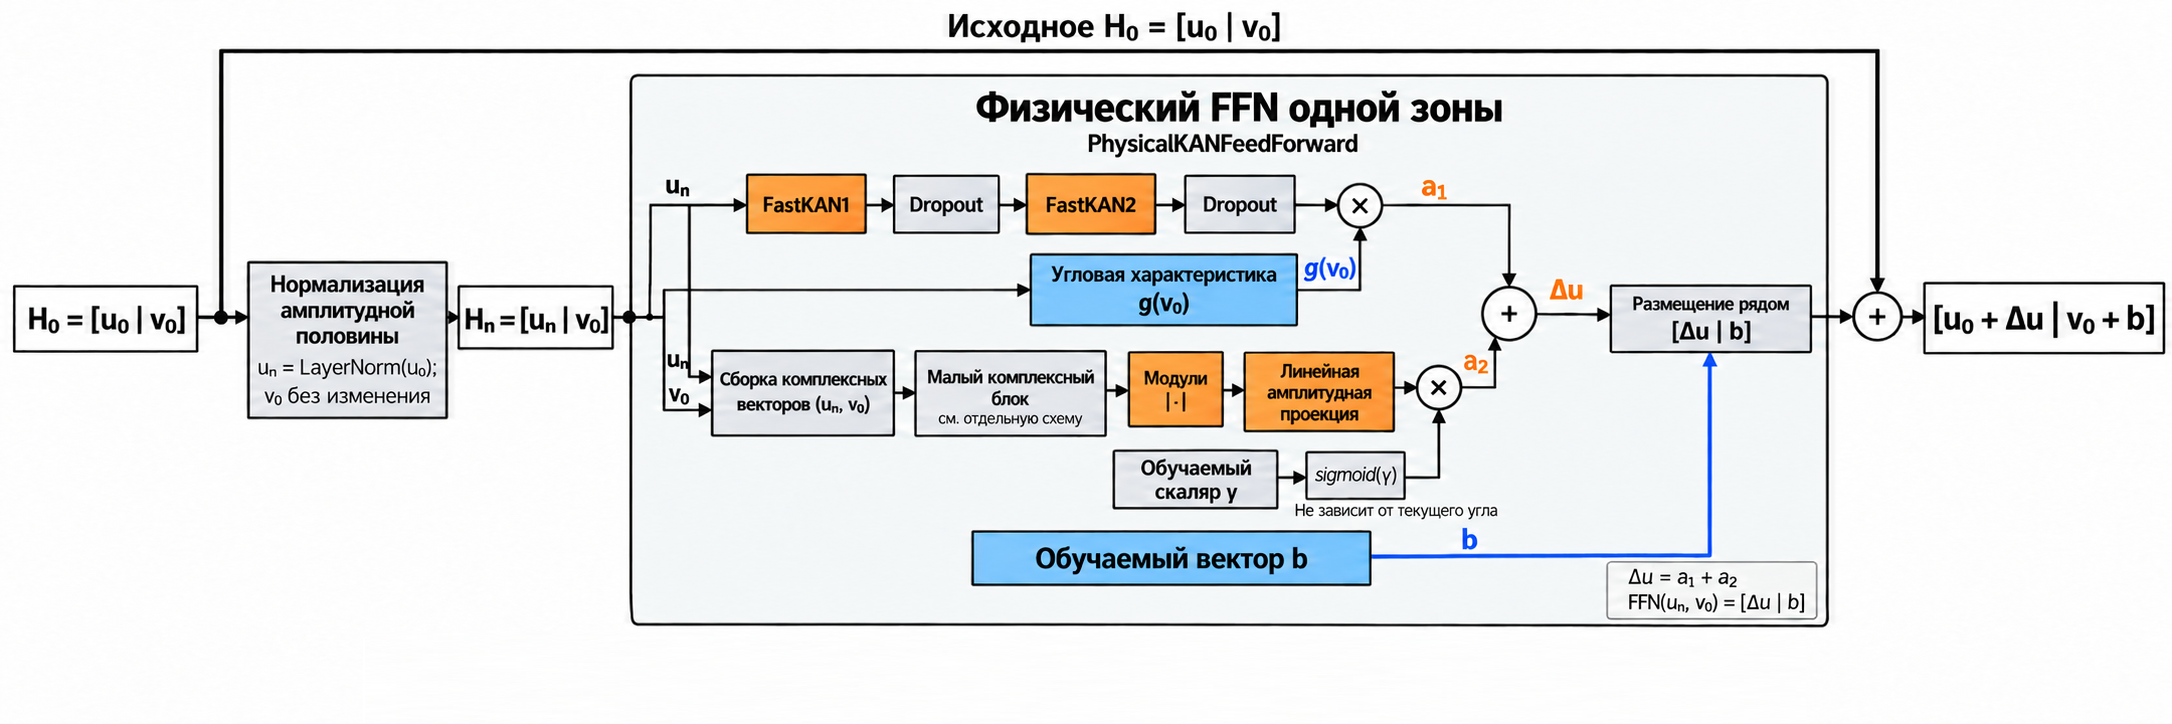
\includegraphics[width=\textwidth]{transformer_ffn_detail.png}
    \caption{Физический FFN и сложение двух амплитудных вкладов.
    Показаны нормализованный вход FFN и обход исходного состояния}
    \label{fig:ch4_physical_ffn}
\end{figure}

\begin{table}[htbp]
\centering\small
\caption{Различие входного каскада и физического FFN}
\label{tab:ch4_physical_code_paths}
\renewcommand{\arraystretch}{1.35}
\begin{tabularx}{\textwidth}{@{}>{\raggedright\arraybackslash}p{0.23\textwidth}>{\raggedright\arraybackslash}X>{\raggedright\arraybackslash}X@{}}
\toprule
Операция & Входной PhysicalStem & Физический FFN \\
\midrule
Управление KAN-ветвью & До FastKAN & После двух FastKAN-слоёв \\
\addlinespace[4pt]
Комплексные результаты & Используются модули и аргументы & Используются модули \\
\addlinespace[4pt]
Объединение амплитудных вкладов & Размещение рядом перед проекцией & Сложение с обучаемым коэффициентом \\
\addlinespace[4pt]
Угловой выход & Проекция исходных и новых углов & Приращение для внешней остаточной связи \\
\bottomrule
\end{tabularx}
\end{table}

\iffalse
(Примечание автора: надо бы как-то добавить, зачем мы вообще разделили эти PhysicalStem и Физический FFN. От части, исходно, это некий косяк и невнимательность, когда оно было применено только на вход, а не в блоки FFN, позже же сделали различие в том, что входной – делает больше таких вот умножений / делений, а в дальнейших, это лишь небольшая функция, которая может быть полезна, ибо математически оно довольно объёмна может быть. Ну и может сейчас ещё есть какие-то существенные отличия, в общем осмысли это – и опиши перед / после данной таблицы, или даже где-то раньше. А то читателю не понятно, с чего вообще это появилось. Про некий косяк в прошлом говорить не надо. Но можно озвучить, что вероятно, такое прям разделение и не требуется. Исходно блоки планировались как нечто одинаковое. Если это сильно не так по итоговым цепям, то надо переосмыслить их, и вероятно менять архитектуру и перезапускать эксперименты и обучения…
И да, повторю ещё раз, исходно должны быть и пропускание токов / напряжения чисто, ну или других величин. Без вот этого вот физического умножения деления, если это не прям так – то косяк! Может обыгрывается через сумму, но вроде бы должно через объединение - конкатенация) **[AA075: закрыто автором; сохранено в истории]**
(Примечание автора: Ок, там пометили вроде бы, пусть пока так, а здесь по тексту примечание закрываем)
\fi
\authorreviewnote{AA075}

Входной каскад и физический FFN используют общую идею
комплексных взаимодействий, но занимают разные места в сети.
PhysicalStem получает измерительные признаки с заданным составом
каналов и согласует их с размерностью скрытого представления.
FFN обновляет уже сформированные признаки после обмена
информацией между зонами. Его вход и выход имеют одинаковую
скрытую размерность, что позволяет повторять такие блоки.
Уменьшенное число комплексных результатов в FFN ограничивает
объём многократно выполняемой обработки.

Различается и способ передачи прежней информации. Входной
каскад размещает рядом отклики KAN и дополнительные модули,
после чего проецирует их. В повторяемом блоке поправка FFN
складывается с прежним скрытым состоянием. Эта остаточная
связь сохраняет прямой путь скрытых признаков, но не создаёт
отдельных неизменных каналов измеренных токов и напряжений.
Конкатенация исходных величин с производными и остаточное
сложение являются разными архитектурными решениями
и в данной работе подробно не изучались.

При включении FFN в повторяемый блок его вход предварительно
нормализуется. В варианте с амплитудной нормализацией изменяется
часть $u$, а часть $v$ проходит без такого преобразования.
Внешний обход передаёт состояние до нормализации. Поэтому
прибавляемая поправка вычисляется из нормализованного входа,
а складывается с прежним состоянием блока. На рисунке
исходное состояние $H_0$ и нормализованный вход $H_n$
обозначены раздельно.

Такая обработка выполняется в каждом блоке с физическим FFN.
Уменьшается число комплексных результатов, а не частота
использования операций по глубине. По умолчанию входной каскад
формирует шестнадцать результатов, из них восемь произведений
и восемь отношений. Каждый физический FFN формирует четыре,
по два каждого вида. Конкретные размеры задаются конфигурацией.

Во входном каскаде операции действуют на измерительные признаки,
а после внимания на их обучаемые комбинации. Скрытые части
проходят проекции, позиционное кодирование и остаточные сложения,
поэтому их нельзя во всей глубине считать неизменными токами
и напряжениями. Направляющий коэффициент регулирует одну ветвь,
а комплексный вклад передаётся параллельно. Это не жёсткая
блокировка всего выхода модели.

После последнего блока выполняются нормализация и подготовка
представлений для выбранной задачи. При зонной классификации
признаки усредняются внутри каждой выходной зоны и поступают
в классификатор. Предобучение использует свой выход реконструкции.
Общее устройство излагается здесь один раз, а обучение, результаты
детекции и проверка требуемого состояния РНМ рассматриваются далее.
Наличие направляющего блока внутри сети не заменяет предметную
проверку органа БАВР в главе~\ref{ch:ml_adaptive_algorithms}.

\paragraph{Варианты для сопоставления.}
Наряду с физическим KAN-трансформером рассматривается
Physical MLP-Transformer. Он сохраняет комплексные взаимодействия
входного каскада и полярное внимание, но вместо входного FastKAN
использует линейное преобразование, а вместо физического FFN
обычный MLP-блок. В таком FFN отсутствуют отдельные комплексная
ветвь и угловое управление, показанные на
рисунке~\ref{fig:ch4_physical_ffn}. Поэтому это сопоставление
затрагивает состав повторяемого блока, а не только способ
задания нелинейной функции. Выходной классификатор также
задаётся конфигурацией.

Базовый трансформер может получать спектральные векторы
либо мгновенные значения токов и напряжений. Во втором случае
меняется состав входа и длина обрабатываемой последовательности.
Влияние входного представления рассматривается отдельно
от изменения физического каскада и нелинейных слоёв.
Обучение и результаты этих вариантов излагаются далее
вместе с использованными конфигурациями.

\subsection{Место архитектурного подхода в исследовании}
\label{sec:ch4_architecture_summary}


\iffalse
(Примечание автора: Возможно тут описать про переход от одной к другой, о чём спрашивал ранее.) **[AA063: закрыто автором; сохранено в истории]**
(Примечание автора: Вопрос решён, закрываем пункт)
\fi
\authorreviewnote{AA063}


\iffalse
(Примечание автора: А про трансформерную модель тут чего не сказано ничего? Надо бы, она ведь от части состоит из того, что было рассмотрено ранее. А так, сей раздел огромным описательно делать не надо, согласен, он кратко описывает итоговые варианты моделей. Может прост добавить, что-то из серии, исследования шли постепенно, и поэтому в работе не приводится везде сравнения сразу для всех исследований, как-то аккуратно об этом) **[AA065: закрыто автором; сохранено в истории]**
(Примечание автора: Описание появилось, сейчас добавим картинки, и потом сравню. Можешь переписать замечание как "провести проверку / сравнение описаний в статьях и тут, может что-то сократишь, а что-то наоборот добавишь, оно должно быть понятно и для людей, кто не работал с трансформерами.")
(Примечание автора: Да, вопрос решён, закрываем его)
\fi
\authorreviewnote{AA065}

Рассмотренные модели образуют несколько связанных вариантов
обработки. MLP, CNN и ResNet задают исходные способы организации
связей. SimpleKAN и ConvKAN позволяют исследовать замену
фиксированных нелинейностей обучаемыми функциями. В PhysicsKAN
к этим преобразованиям добавлены произведения и отношения
сигналов, cPhysicsKAN переносит операции в полярное представление,
а rPhysicsKAN вводит отдельный направляющий орган. Последние
варианты связаны общей идеей, но не являются обязательными
последовательными ступенями одной сети. Каждый из них может
обучаться и сравниваться самостоятельно. Physical KAN-Transformer
использует эти физические операции и направляющее управление
при анализе последовательности механизмом внимания.
Исследования развивались постепенно, поэтому состав сравниваемых
моделей и протоколы в разных опытах различаются. Совокупность
этих опытов не является одним сравнением всех архитектур
на неизменном наборе данных.

При сопоставлении вариантов используются общие правила оценки
из раздела~\ref{sec:ch4_evaluation_methodology}. Представления сигналов
и условия обучения рассматриваются далее отдельно от устройства сети.

Подготовленные в главе~\ref{ch:dataset_preparation} данные
дают основу для исследования этих моделей на реальных
процессах. Объяснение архитектуры определяет, каким образом
используются сигналы, а сравнение на согласованных выборках
позволяет оценить результат этого выбора. Последующая
проверка конкретного измерительного органа связывает
нейросетевой подход с совершенствованием алгоритмов БАВР.
